\documentclass[a4paper,11pt,column]{article}
\usepackage[latin1]{inputenc}
\usepackage[english]{babel}
\usepackage{amsmath}
\usepackage{amsfonts}
\usepackage{amssymb}
\usepackage{cuted}
\usepackage{pdfpages}
\usepackage{mathpazo}



\usepackage{titling}
\usepackage{siunitx}
\usepackage[style=ieee,backend=bibtex]{biblatex}
\addbibresource{designbib.bib}
\usepackage[font={small}]{caption}
\usepackage{subfig}
\usepackage{nomencl}
\makenomenclature





\usepackage{graphicx}
\usepackage{color}

\usepackage{booktabs}
\usepackage{threeparttable}
\usepackage{fancyhdr}
\usepackage{float} %floats are used to contain things that must be placed inside a single page

\usepackage{varioref}
\usepackage{textcomp}
\usepackage{xspace}
\usepackage[activate={true,nocompatibility},final,tracking=true,kerning=true,spacing=nonfrench,factor=1100,stretch=10,shrink=10]{microtype}




%---------------------------------------------------------------------------------------------------------------------------------------------------------------------------------------------------------
% Document Information
%---------------------------------------------------------------------------------------------------------------------------------------------------------------------------------------------------------
\author{Group 25}
\title{Design Report}
\date{\today}

% Path to images.
\graphicspath{Images}

% Header and footer.
\pagestyle{fancy}
\fancyhf{}
\lhead{\thetitle}
\rhead{\theauthor}
\cfoot{\thepage}
\renewcommand{\headrulewidth}{0pt}
\renewcommand{\footrulewidth}{0pt}

\begin{document}


%% Title page.
\begin{titlepage}
    \centering
    \vspace*{\fill}
    
\includegraphics[width=\textwidth]{Images/Durham.jpg}
    \vspace*{\fill}
    \LARGE\thetitle\\
    \large\theauthor\\
    \large Professor PH Gaskell, Keith Blundy\\
    \large L2 Design\\
    \large\thedate\\
    \vspace*{\fill}
\end{titlepage}

%---------------------------------------------------------------------------------------------------------------------------------------------------------------------------------------------------------
% Main matter.
%---------------------------------------------------------------------------------------------------------------------------------------------------------------------------------------------------------
\onecolumn 
\section{Executive Summary} 
Microphonic effects exist in hi-fi systems wherein mechanical vibrations are transformed into unwanted electrical signals, termed noise, that consequently reduce sound quality. Isofonics have designed footers of aluminium and steel upon which such systems are to be supported that aim to isolate and attenuate the signals responsible for this aforementioned noise. Three footers are required per system, three being the minimum number of points of contact necessary to support a rigid mass, and are to be sold as a device comprising a contained magnetic damping mechanism with two optional additional pieces; a removable base to use the device as a stand alone mount as opposed to its mounting within existing equipment and a removable spike offering a minimal point of contact. The main device, base and spike are to cost �blah, �blah and �blah respectively, placing Isofonics at the higher end of the existing market due to its premium quality components embodying a design that is both innovative and effective. The device may be altered manually by the user to support a range of different masses, a feature of customisability unique to Isofonics. This process may also be informed by a user friendly phone application. Additionally, within this design lies potential for product families of differing size, catering to an even wider audience, and applications within the field of optics, more specifically in the optimisation of microscopes.
%Sufficient information to give an appreciation of the problem being addressed, the proposed solution and any relevant information on cost, application or other major aspects that would concern decision maker%

%acronyms
\nomenclature[A0]{DFM}{Design for Manufacture}
\nomenclature[A1]{DFA}{Design for Assembly}
\nomenclature[A2]{CNC}{Computer Numerical Control}
\nomenclature[A3]{URS}{User Requirement Specification}

%Variables
\nomenclature{test}{This is a test}

\printnomenclature

\tableofcontents

\section{Introduction}
Microphonics describes the phenomenon wherein internal components within an electronic device transform mechanical vibrations into undesired electrical signals\cite{microphonics}. In the context of hi-fi systems, and when these vibrations are within the frequency range audible to the human ear (20 Hz - 20 kHz), they equate to noise that reduces audio quality and therefore threatens the user\textquotesingle s listening experience. This report details the design of vibration isolation and attenuation mounts that minimise this interference as well as that originating from external sources. 
\\\\The following function analysis tree defines the user requirement specification for the product:

\begin{figure*}[h]
   \centering
   \includegraphics[width=\textwidth]{images/URSTree}
   \caption{User Requirement Specification Diagram}
   \label{}
\end{figure*}


With such a niche product consisting of high tolerance machined parts and premium materials comes a high cost, indicating a corresponding market; middle aged/mature clientele with strong technical understanding of the hobby and its principles or affluent younger hobbyists. The current market offers a range of mounts at a range of prices within which our product shall lie at the higher end, namely between �1500- �2000 per mount. 
Market leaders such as Stillpoints\textsuperscript{\textregistered}, Nordost\textsuperscript{\textregistered} and Isoclear\textsuperscript{\textregistered} offer sleek solutions yet lack the tailorability offered by our design, allowing customers to pre-load their mounts manually for individual amps, potentially with interactivity provided by an instructive technical app (see section blah). After conducting market research via surveys, it was found that potential customers were very much interested in the ability to manually adjust their mount as appropriate and that this offered an invaluable, unique selling point.
\\This report covers the initial design concepts proposed by Group 25, the development of a chosen design, its design for manufacture and sustainability and, briefly, its commercial considerations. 


\section{Design Concepts} 
%Describe alternative approaches to a solution and
%explain how one particular approach was selected.


\section{Design Development} 

\subsection{Parametric Model} 


\subsection{Dynamic Model}  %MAT
\subsubsection{Why use a Dynamic Model?}
It was determined that a dynamic model of the system would be necessary to quantify the potential success of the product. This could visually display the effects of the footers on attenuation of a signal from a Hi-fi system, and hence establish whether the sound quality had been improved. 

\subsubsection{Forming the Equation}
The system can be simplified to a spring mass damper system; a driving force (Fd(y)) is supplied by the vibration of the Hi-fi system and the opposing forces from the magnetic repulsion force (Fm(y)) and damping coefficient (c). Considering these components, it was possible to develop a second order differential equation (see equation \ref{eq:2ndDiff}) which when solved would characterise the function of the footers.

\begin{equation} \label{eq:2ndDiff}
Fd(y) -my^{\prime \prime} - cy^\prime - Fm(y) = 0 
\end{equation}
as defined in \cite{2DoF}.

Where m is the mass of the system and y is the displacement due to vibrations.

Three components were to be found to complete the model; c, Fd(y), and Fm(y).
From the parametric modelling, the damping coefficient was calculated (EQUATION XXX FROM BENEDICT) for an amplifier of 20kg using an estimated value of the coefficient of friction (?) ranging from 0.4 to 0.6. This gives a range for the damping coefficient:

c = 158.7182 Ns/m for	? = 0.4
c = 238.0773 Ns/m for	? = 0.6							

The value of the magnetic repulsion force can be calculated, as outlined in section XXXX using equation XXX. The repulsion force is driven by the horizontal movement of the ball bearings; this motion is directly proportional to the vertical displacement from vibrations.

Figure~\ref{fig:CrossSection} displays a cross-section of the footer, the separation of the magnets, M12, moves with length z, and z relates to y via equation \ref{eq:z}.

\begin{figure*}[h]
   \centering
   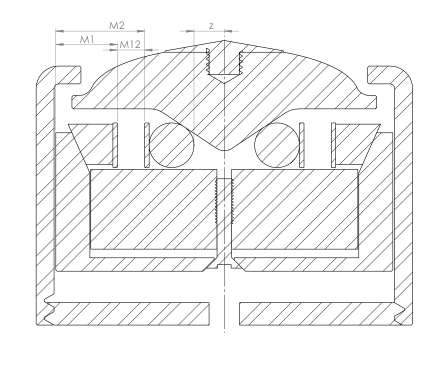
\includegraphics[width=0.5\textwidth]{images/Mat1}
   \caption{Footer Cross-Section}
   \label{fig:CrossSection}
\end{figure*}


\begin{equation} \label{eq:z}
z = y (w/h) 	
\end{equation}

Where w and h are the dimensions shown in figure ?WHAT FIGURE?
The final element of the differential equation to consider was the driving force from vibrations; this is simply calculated by Newton?s Second Law of Motion, equation \ref{eq:Newton}.

\begin{equation} \label{eq:Newton}
Fd = my^{\prime \prime}
\end{equation}

The mass of the system (m) is easily found, however the acceleration of the vibrations $y^{\prime \prime}$ must be found empirically; sample data was needed.

\subsubsection{Experiment}
%start experiment section
\subsubsection{Intro}
To model the effectiveness of the product, sample data was collected to act as an input for the model; this data was used to simulate the driving force in the characteristic equation previously stated (Equation \ref{eq:2ndDiff}).  In order to obtain this information, an experiment was completed.

\subsubsection{Experimental Method}
A 5V signal was generated with a PicoScope (pico Technology, PicoScope 2204A) and fed through an accelerometer (STMI electronics LIS344ALH); this accelerometer was coupled to the top of an amplifier connected to a standard AC mains power supply, nominal voltage of 240V at a frequency of 50Hz. Using the pico Technology software, data from the accelerometer was captured for three conditions; the amplifier turned off, the amplifier turned on, and the amplifier turned on sitting on four half squash balls placed under the footers. Squash balls are a rudimental method of noise damping and were tested to compare this known method against the information acquired from the mathematical model.

The data captured came in the form of a voltage output, to determine the acceleration from this information it was necessary to form a transformation equation. To do so, the technical data sheet for the accelerometer was found and in it there was clear conversion data which lead to the following

\begin{equation} \label{eq:acceleration}
a  =  (0.66 V - 1.65) 9.81
\end{equation}

as derived from \cite{SensorManual}

Where a is the acceleration $(ms^{-2})$, V is the voltage response from the accelerometer (V).

With the acceleration response and the mass of the amp, the driving force from the vibrations was calculated (Equation \ref{eq:Newton}) for each of the conditions.
%end experiment section 

\subsubsection{Data Processing - FFT}
Once the sample data was captured, it needed to be processed to allow for further analysis. A Fast Fourier Transform (FFT) takes a signal, the driving force from vibrations for example, and breaks it up into a combination of simple waves; with this decomposition, it is possible to represent the data in the frequency domain rather than as a time series. To accomplish this an FFT script was written in MatLab, this was applied to the experimental data.

Firstly, the data for the amplifier off, the control, was compared to the amplifier on. Both sets of information were processed and their spectra plotted as shown in Figure \ref{fig:MatGraphs1}

\begin{figure*}[h]
   \centering
   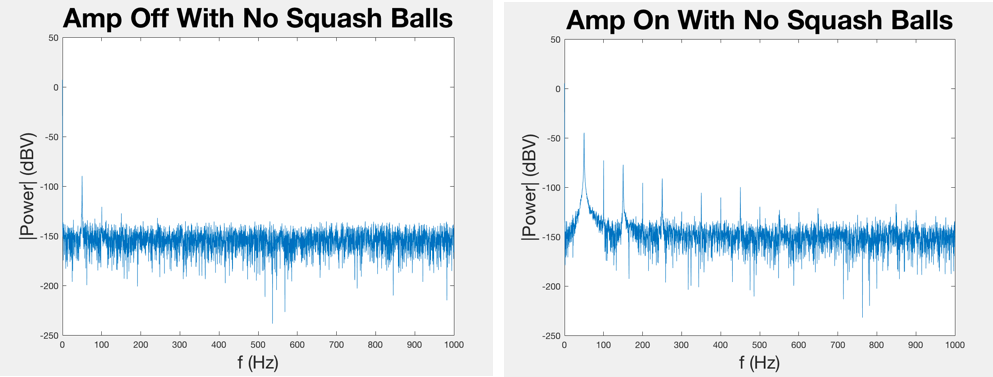
\includegraphics[width=\textwidth]{images/MatGraphs}
   \caption{Compared Frequency Responses when Amplifier off and on}
   \label{fig:MatGraphs1}
\end{figure*}

The amp off data has a thin peak at 50Hz; this is due to the UK mains power supply rated at 50Hz. Although the amplifier was turned off it was still connected to the mains and therefore it is not unusual to witness a peak. With the amplifier on the fundamental frequency increases in power significantly up to -40dBV from -130dBV. The harmonics can be seen at 50Hz intervals although the general noise of the signal remains the same. Next, the amplifier on data was compared to the squash ball damped data to show how rudimental damping will affect the spectra and indicates how to determine successful damping for the dynamic model. The graphs are shown in Figure \ref{fig:MatGraphs2}

\begin{figure*}[h]
   \centering
   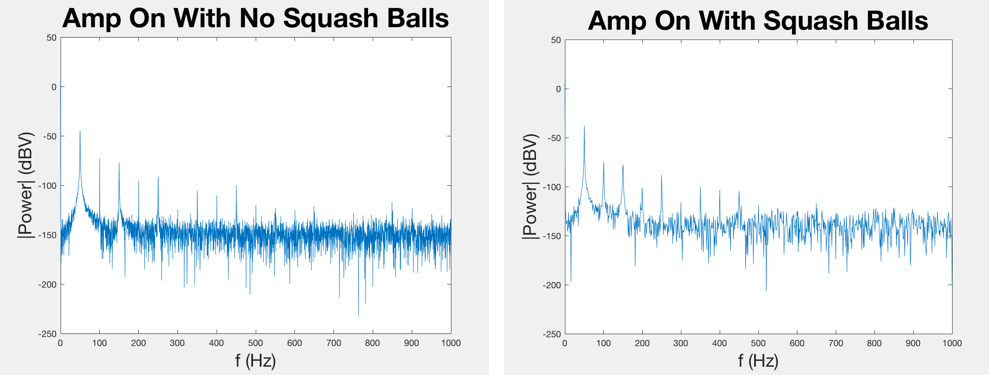
\includegraphics[width=\textwidth]{images/MatGraphs2}
   \caption{Compared Frequency Responses with and without Squash Balls}
   \label{fig:MatGraphs2}
\end{figure*}

From the undamped spectra, it can be observed that the fundamental frequency is 50Hz with a peak at around -50dBV and harmonics at 50Hz intervals. There is heavy noise on the spectrum which will need to be reduced to provide an improved sound quality. From the simple damping the squash balls provide this noise has been significantly attenuated, along with this success the harmonics have consistently lower peaks whilst the fundamental frequency retaining a similar power to the undamped spectrum. This provides an example of successful damping which can be used as a comparison to the later mathematically damped data. The aim is to further reduce the noise and lower the power of the harmonics as much as possible, preferably below the noise floor which can be observed to be around -130dBV.

\subsubsection{Choice of Software- Simulink}
Simulink was chosen to drive the dynamic model due to the straight-forward construction of differential equations it provides; it offers a visual representation of the system and works hand-in-hand with MatLab allowing for simple data processing. Simulink computes an iterative numerical solution and outputs a corresponding time series to the MatLab workspace.

\subsubsection{Modelling Process and Driving Equations}
The first step to modelling was to consider each element of the characteristic equation and form a series of blocks to represent them. The output from MatLab represented the acceleration from the accelerometer ($y^{\prime \prime}$) therefore two \textquotesingle integrator\textquotesingle blocks were used in series to provide branches for $y^{\prime}$ and y. Each of these branches were then routed and manipulated to determine their effects on the equation.
Figure \ref{fig:MatModel} displays the final form of the model.

\begin{figure*}[h]
   \centering
   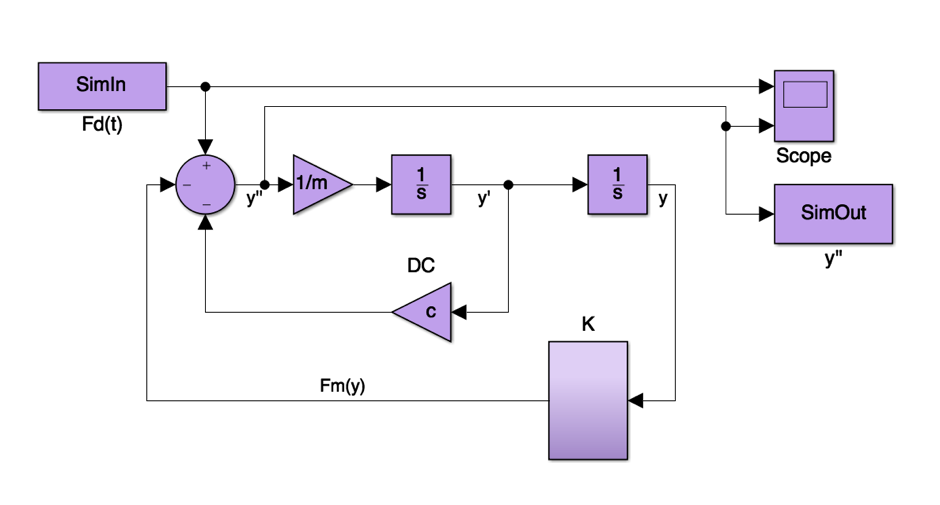
\includegraphics[width=0.8\textwidth]{images/MatModel}
   \caption{Compared Frequency Responses with and without Squash Balls}
   \label{fig:MatModel}
\end{figure*}

\textquotesingle SimIn\textquotesingle provides the experimental data from the MatLab workspace and similarly, \textquotesingle SimOut\textquotesingle exports the mathematically damped data; \textquotesingle Scope\textquotesingle displays the input and output data together in the time domain. The triangular blocks multiply the branch by a constant stored in MatLab; \textquotesingle K\textquotesingle is a subsystem modelling the equation for magnetic repulsion force for a given displacement, y. These branches summed together as shown by the circular block will simulate the differential equation and hence the damping from the footers.

\subsubsection{Simulating Damping}
The driving force calculated from the experimental data was used as the input for the dynamic model; the value of damping coefficient is constant and the magnetic damping varies as the displacement of the data changes. A Fourier Transform was applied to the output of the model to analyse the spectrum. The \textquotesingle Amp on\textquotesingle data is used as the input for the system and Figure \ref{fig:CoF} displays the output spectra for the values of damping coefficient at the lower and upper bound values of coefficient of friction.

\begin{figure*}[h]
   \centering
   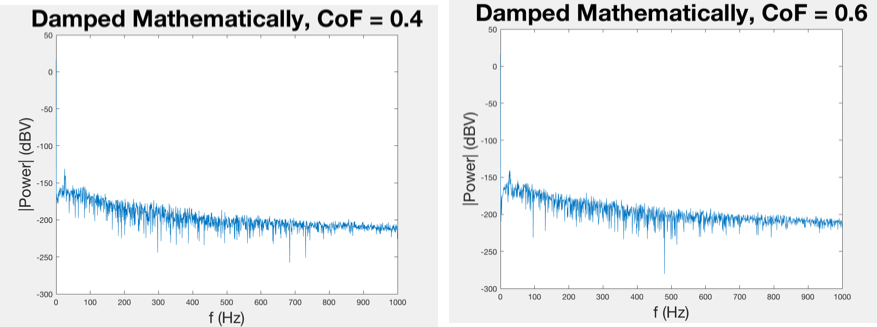
\includegraphics[width=\textwidth]{images/MatGraph3}
   \caption{Power Output for Coefficient of Friction Extremes}
   \label{fig:CoF}
\end{figure*}
















%dimension selection- bearings driving dimensions, tracks, screws

%Pre-load system- maths behind pre-load weights, check torque manageable, effect of pre-loading on mass and nat freq & damping factor, magnet dimensions,bearings

%selections of materials- steel durable, contain flux


%(Describe the development of the design to
%determine say the principal dimensions or weights,
%selection of materials)

\section{Detail Design} \label{sec:DetailDesign}

%(Describe the minor details, such as nuts and bolts, - RUSSELL
%details for avoiding stress concentrations suitability of screws,-GEORGE specify any bought-in
%components.)
 
\section{Design for Manufacture} 

DFM defines the design/engineering of a product so as to best optimise its quality whilst minimising its cost to manufacture\cite{dfm}. Factors affecting this cost include the number of off-the-shelf and machinable parts, the set-up time of required machinery, the material type, dimensional tolerances as well as secondary processes. Generally, a compromise is reached between the functional quality of a product and the cost of manufacture however, considering the current extortionate pricing of similar existing products, certain design choices have taken precedence over their implications in a manufacturing context, for the example the complex central piece (see drawing COR080-0003).

\subsection{Off-The-Shelf Parts}
Due to the complex geometry required from our design, only few components may be bought in, namely (per mount);  six �10mm tungsten carbide ball bearings, six �10 x 1.5 mm neodymium magnets, six M4 by 20 mm AISI A2 steel countersunk Torx security screws and one M4 by 20 mm countersunk hex socket with partial thread. These components are readily available excluding the tungsten carbide ball bearings which must be sourced from a specialist supplier.
Table~\ref{table:BoM} details potential sources for the aforementioned parts and their corresponding cost.


\begin{table}[h]
	\centering
	\caption{Bill of Materials}
	\begin{tabular}{@{}rp{9em}p{9em}rrr@{}}
		\toprule
		Item No. & Part No. & Description & Qty. & �/Piece & � Total \\
		\midrule
		1 & COR080-0003 & Isofonics core & 1 & --- & --- \\
		2 & PLD080-0003 & Isofonics preloading crown & 1 & --- & --- \\
		3 & PLD010-1004 & Isofonics preloading backstop & 6 & --- & --- \\
		4 & F669-N45SH-10 (first4magnets) & 10 x 1.5mm neodymium magnet & 12 & --- & --- \\
		5 & 10MMTUNGSTENB ALLS (VXB Bearings) & 10mm tungsten carbide ball & 6 & --- & --- \\
		6 & TOP080-0004A & Isofonics top piece & 1 & --- & --- \\
		7 & RET080-0003 & Isofonics retainer & 1 & --- & --- \\
		8 & M4X20-CSK-ST (westfieldfasteners) & Partially threaded M4 x 20mm c'sunk security screw & 1 & --- & --- \\
		9 & M4X20-CSK-H (westfieldfasteners) & Partially threaded M4 x 20mm c'sunk hex socket screw & 1 & --- & --- \\
		10 & USR080-0001 & Isofonics removable spike & 1 & --- & --- \\
		11 & RET080-1002 & Isofonics retainer bottom & 1 & --- & --- \\
		12 & USR080-1002 & Isofonics removable base & 1 & --- & --- \\
		\bottomrule
\end{tabular}
\label{table:BoM}
\end{table}


\subsection{Machined Parts}
All other parts may be machined using a 3 axis CNC mill excluding the central piece (see drawing COR080-0003), which requires 4 axis machining. 4 axis machining is substantially more expensive but allows for more intricate designs by using a 4th axis to reposition the part between 3 axis operations, a feature required for this design\cite{cnc}.

\subsubsection{Set-up Time}
Cost is substantially driven by time; time to remove material in the machining process as well as set-up time of the machine itself\cite{SetUp}. Conveniently, our design is highly symmetrical meaning time and money is saved through lacking the need of a complex orienting mechanism given that the part's orientation prior to machining is irrelevant.

\subsubsection{Material Type}
Steel is harder, and therefore more expensive, to machine than softer materials however, its properties make it invaluable to the quality of the product (see Section~\ref{sec:DetailDesign}) and pose no problem for the advanced machining capabilities of today. The product's entire composition out of steel was initially proposed but after receiving a quote from 'Sylatech' (r/c), a machining company in the northeast of England for �---- per piece, it was evident some optimisation was required to quote a retail price for our product that allowed for a 35\% \cite{ProfitMargins} profit margin.For this reason, it was decided that all non-critical parts may be machined from aluminium, an alternative roughly 1.5 times cheaper\cite{AluVSteel} than steel. 'Non-critical' in this context refers to all parts excluding the complex central piece (COR080-0003) for which steel is required to contain magnetic flux leakage and remain unaffected by frictional effects of the moving bearings. Additionally, aluminium is roughy 5 times easier to machine than stainless steel\cite{AluVSteel} saving significantly on time, and therefore cost.

\subsubsection{Tolerances}
Initially all parts were to be machined at fine linear and angular tolerances of +/-0.1mm and +/-$1\,^{\circ}\mathrm{}$ respectively to ensure the overall quality of the product. However, in the interest of reducing cost, it was concluded that the rails contained in the core piece are the only parts to be machined to a high tolerance since they are to fit plush to the bearings; all other parts may be machined to a lower, and therefore cheaper, tolerance of +/- xmm.

\subsection{Secondary Processes}
\subsubsection{Finishings}

A 2J finish (brushed finish) has been chosen as it is cheaper to produce than polishing and is practical in that it is resistant to scratches whilst being aesthetically pleasing.

\subsection{Volume}
Finally, the volume of production is of great importance; with too small a batch size, set up costs and jig production costs become impractical and with too large a batch, storage costs pose a problem. Considering the high cost and exclusive appeal of this product, low volume batch production in the order of 100 is appropriate so as to eliminate any unnecessary storage costs.


\subsection{Optimisation}
 %the core may be machined in separate parts that are later joined to avoid the complexity of machining the reverse chamfers as shown in Figure~\ref{fig:core}.

\begin{figure*}[h]
   \centering
   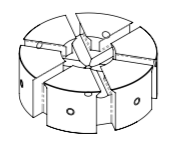
\includegraphics[width=0.3\textwidth]{images/core}
   \caption{Core}
   \label{core}
\end{figure*} 


%what tools are required - allen (purple engraved) , 
%can the design be altered slightly to
%improve convenience and hence cost of
%construction? - smaller less tracks (although crisitcal size exists), split base solid part into separate parts to join, difficults part from reverse chamfers so have one solid base and join blobs.
%parts- 1 top, 1 spike, 12 magnets, 1 retianer, 6 M4 by 20mm countersunk torx security screws, 1 M4 by 20mm countersunk hex socket with partial thread, 1 insert, 1 bottom,1 base, 6 adjustables per batch, jig, jig sleeve
%Can a few common components be used rather than many different varieties?- no, high budget
%
\section{Design for Assembly} 
Due to the small scale of our product, hand assembly is required. Considering the complexity of the design and physical impracticality of overcoming the repulsive magnetic forces during its assembly, a jig has been designed, as shown in drawings JIG080-0001 and JIG080-1001, with full accompanying assembly instructions (see Isofonics Assembly Instructions ISO080-INS).

\begin{figure}[h]
    \centering
    \subfloat[Assembly Jig Base]{{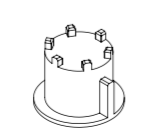
\includegraphics[width=0.4\textwidth]{images/jigbase} }}%
    \qquad
    \subfloat[Assembly Jig Sleeve]{{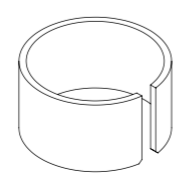
\includegraphics[width=0.3\textwidth]{images/jigsleeve} }}%
    \caption{Assembly Jig Components}
    \label{fig:JigAssembly}
\end{figure}



\section{Design for Sustainability} 
%machined material, scrap of which can be melted purely
%scrap from machinery is recyclable
%possibility to carbon offset the production of products given extortionate pricing 
%longevity of product 

%Have you considered using sustainable materials
%or processes in your design? Can you make it out
%of recycled, novel, or plant-based materials? Can
%it be recycled itself?

\section{Commercial Considerations} 
%Have you included a full Bill of Materials? (george)
%What are the major costs of materials and components? labour and tooling need carbide tools for steel (eloise)
What does it cost to machine parts- (Eloise)
% What is the life of the product before a new model has to be introduced and how many units can be sold in that
%period?- tracks and cone, lifetime magnets, on lubricant, pre-loading

 
 \subsection{Stillpoints Patent Check}
 
 The Stillpoints patent details the design of a \lq{device for the control of vibrations comprising a retainer resting on a base and a plurality of bearings disposed within the retainer}\rq \cite{Stillpoints}within which \lq{the bearings are arranged in at least two layers}\rq \cite{Stillpoints}. It alludes to multiple alternative designs including an \lq{embodiment}\rq in which magnetic fields are employed, however differently to the usage detailed in our design. After studying the official claims made at the end of the patent it is concluded that in not featuring layers of bearings and using opposing magnetic fields as the main damping method, our design differs significantly from the design and alternatives claimed by Stillpoints.\\
 \textbf{It is worth noting this is a US patent and is not filed with the European Patent Office and so only stands to limit sales within the US}
 
 \subsubsection{Parallels with Stillpoints}
 The following details the main claim made by Stillpoints and highlights areas of concern:

\lq{A device for the control of vibrations comprising:
\textbf{a retainer}, the retainer constructed and arranged to rest upon a base, at least a \textbf{portion of the base defining a substantially flat surface}; and \textbf{a plurality of bearings disposed within the retainer, the bearings arranged in a first layer and a second layer}, the second layer disposed on the first layer, the first layer
comprising three or more bearings, and the second layer comprising at least one bearing, each bearing in
the first layer constrained on its bottom by only the substantially flat surface of the base, on its side by the
retainer, the bearings in the first layer supporting the at least one bearing in the second layer, the retainer defining a surface which is in substantially tangential contact with the bearings in the first layer}\rq\cite{Stillpoints}.

It is clear that the main claim focuses on the use of layers of bearings, in this way, our design is fundamentally different. Since our design differs from that outlined in the main claim, all further claims based on the first are irrelevant. An element of originality of our design lies in the use of magnets which is not mentioned at all within the official claims section of the patent.

The use of magnetic fields is mentioned during the preamble and is as follows:

\lq{In some embodiments the first base member 119 and second base member 123 may have opposing magnetic fields.}\rq\cite{Stillpoints}

\begin{figure}[h]
    \centering
    \subfloat[Stillpoints Mechanism Diagram]{{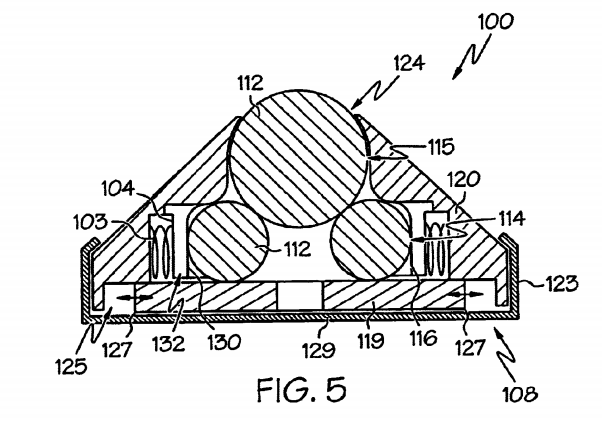
\includegraphics[width=0.4\textwidth]{images/Stillpoints} }}%
    \qquad
    \subfloat[Group 25 Mechanism Diagram]{{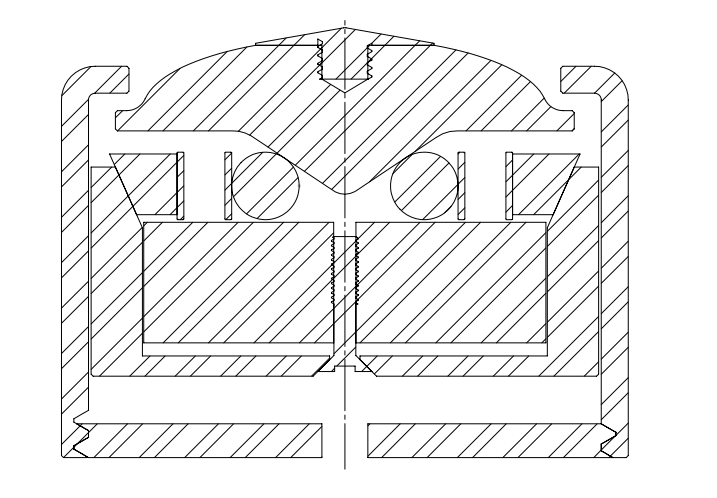
\includegraphics[width=0.4\textwidth]{images/Group25} }}%
    \caption{Stillpoints Mechanism Comparison}
    \label{fig:Patent}
\end{figure}
As can be seen from Figures 1 and 2 , this comment is entirely unrelated to the use of opposing magnetic fields to essentially replace the spring mechanism shown above and consequently does not affect our design.

Figure ~\ref{fig:Patent}

\subsubsection{Points of Originality}
-Use of \textbf{opposing magnetic fields} for lateral damping as opposed to springs\\
- \textbf{Cone with retaining flange} replacing layers of bearings\\
-\textbf{Pre-loading mechanism} in which a screw in tension moves a fixed magnet decreasing its distance from the bearing magnet thus increasing the strength of the system (adjustable for a variety of masses)

\section{Discussion} 
%Discuss the advantages of the proposed design in comparison with alternatives. Discuss how well the design meets the original specification. - Lauren, refer to tree

\subsection{further developments}
%Discuss potential further developments. -
%Discuss the impact on the design of new materials - cheaper with aluminium
%Discuss uncertainties and assumptions in the design process and indicate what practical measurements might be required to give the necessary data to improve the design. - measure damping coefficient, 3d modelling

\section{Conclusion} 
%The conclusions should be a set of brief
%statements of the main results of the project.
%Sometimes bullet points can be used to give
%emphasis


%-----------------------------------------------------------------------------------------------------------------------------------
% REFERENCES
%-----------------------------------------------------------------------------------------------------------------------------------
\section{References}
\printbibliography
%-----------------------------------------------------------------------------------------------------------------------------------

\cleardoublepage
\appendix
\section{Project Plan and Members' Contributions} 
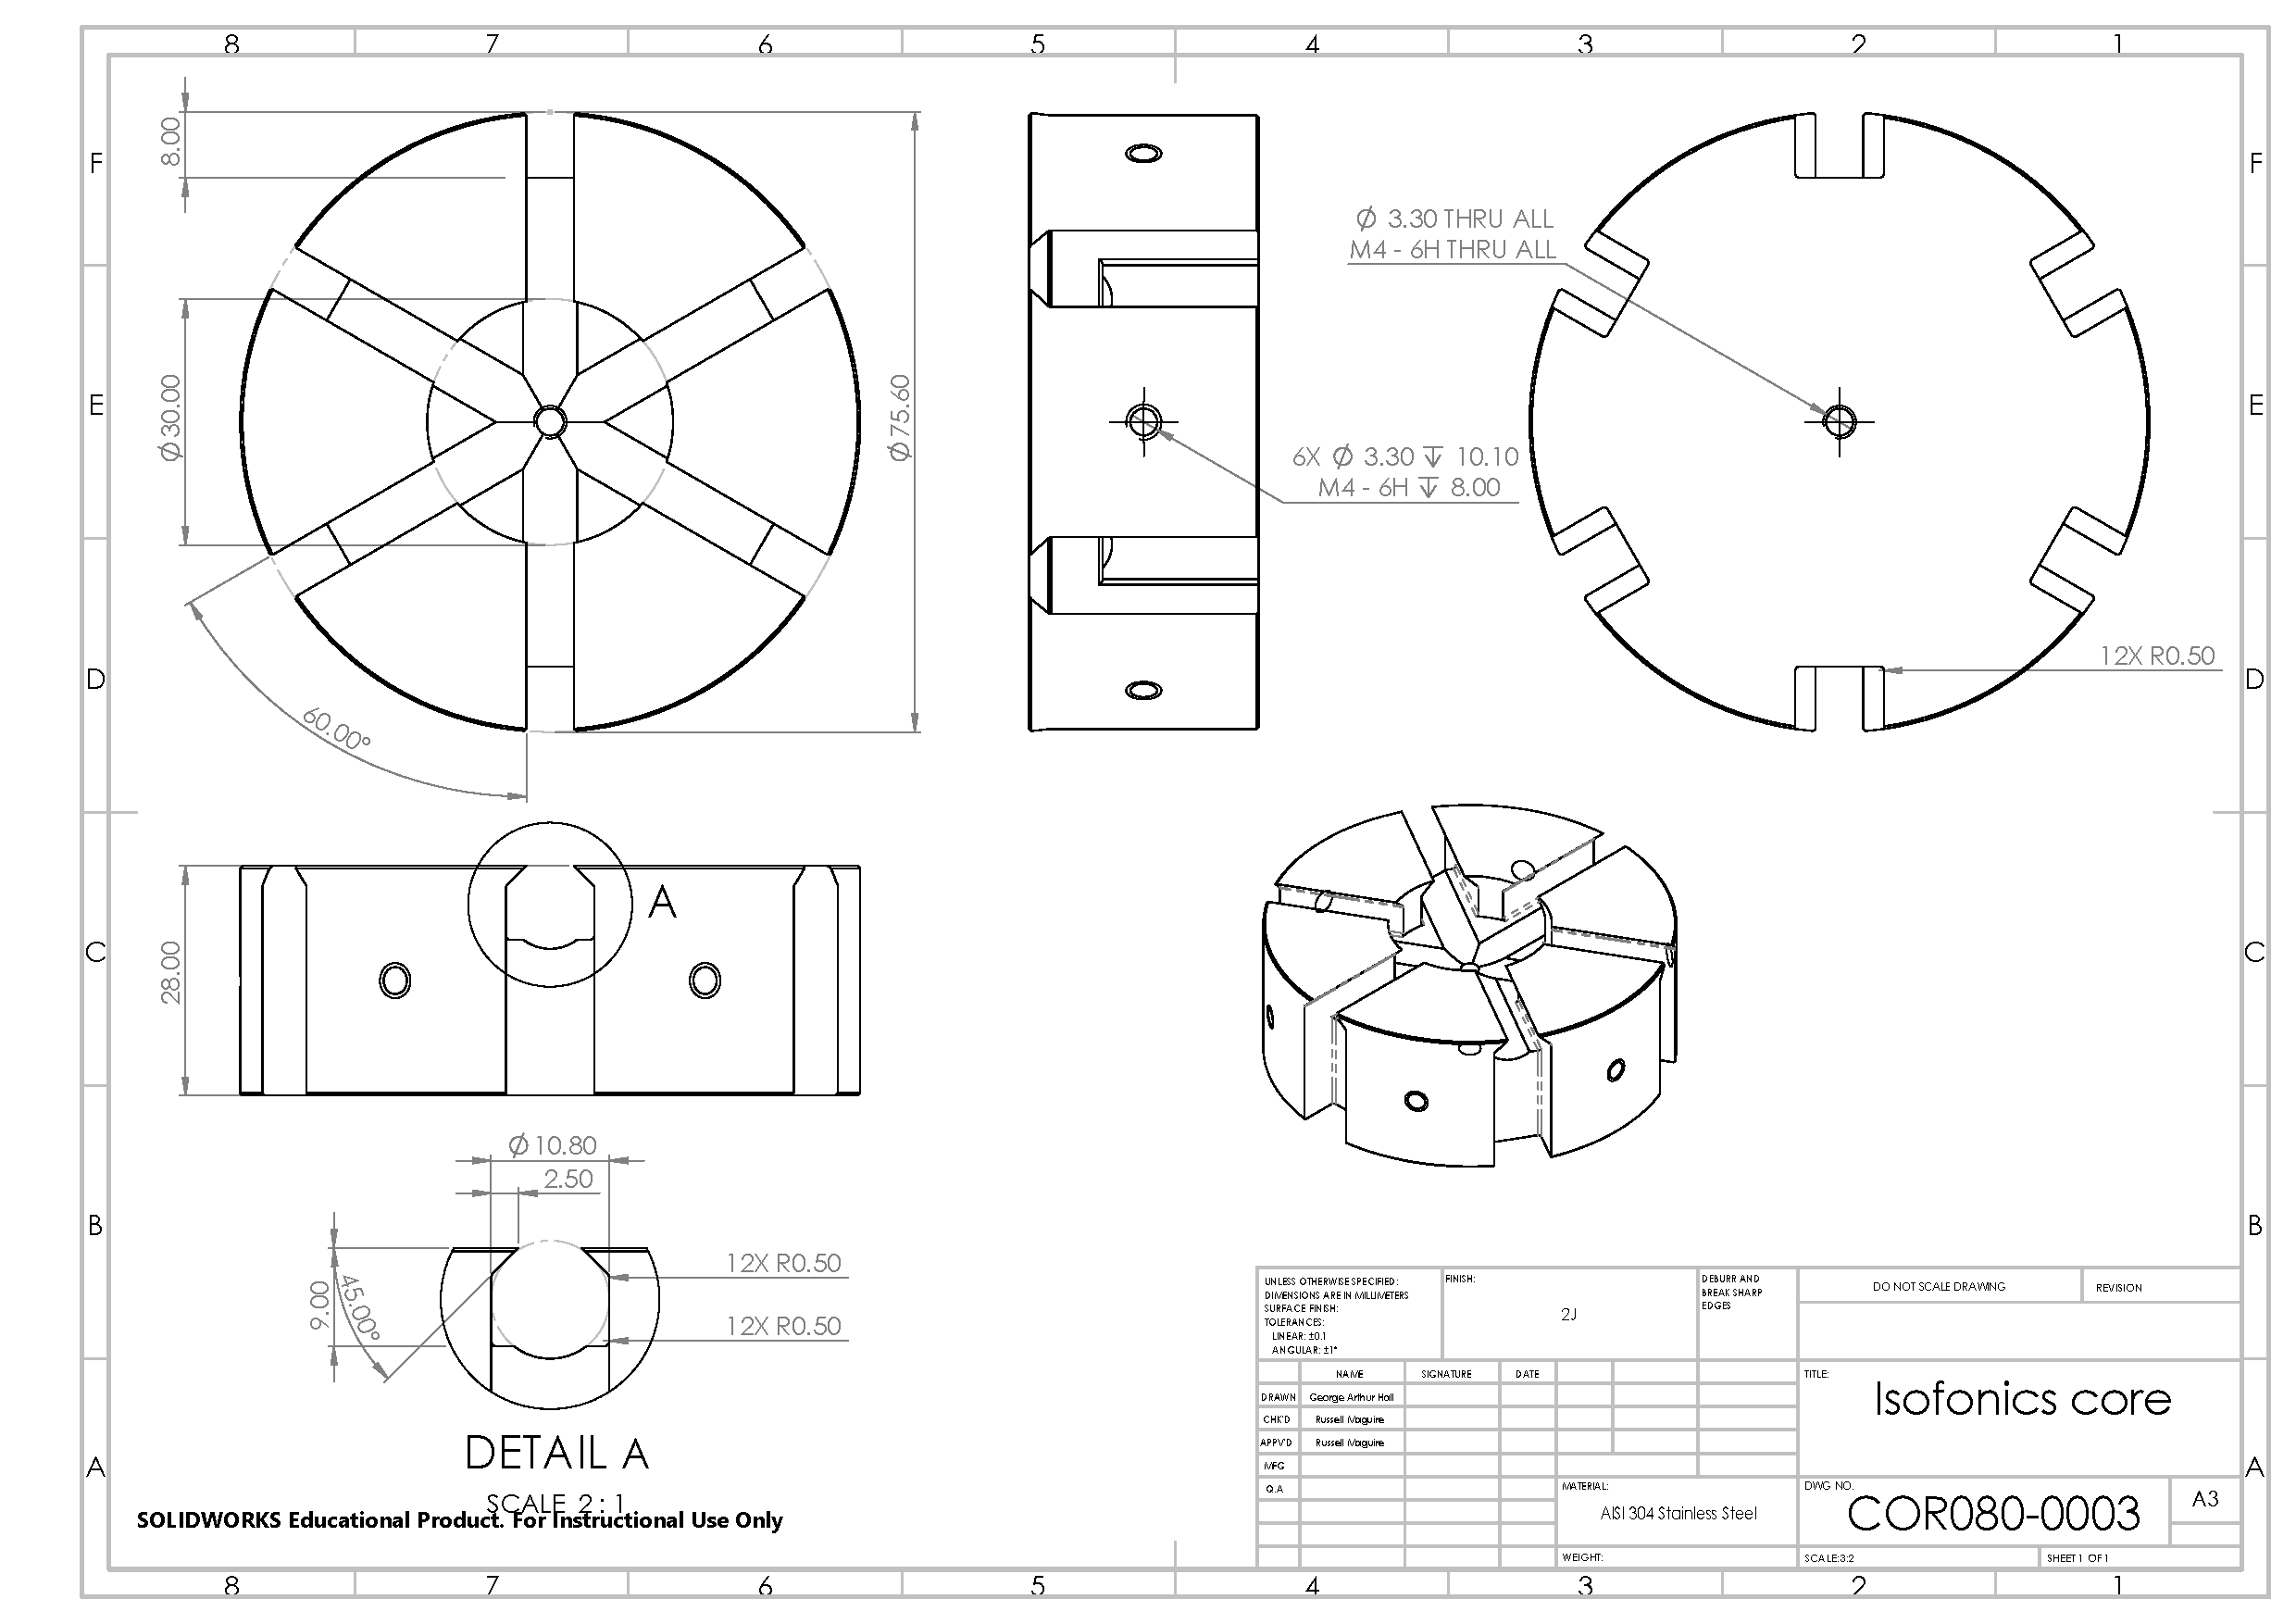
\includepdf[pages=-,fitpaper=true]{Images/Drawings/COR080-0003.PDF}
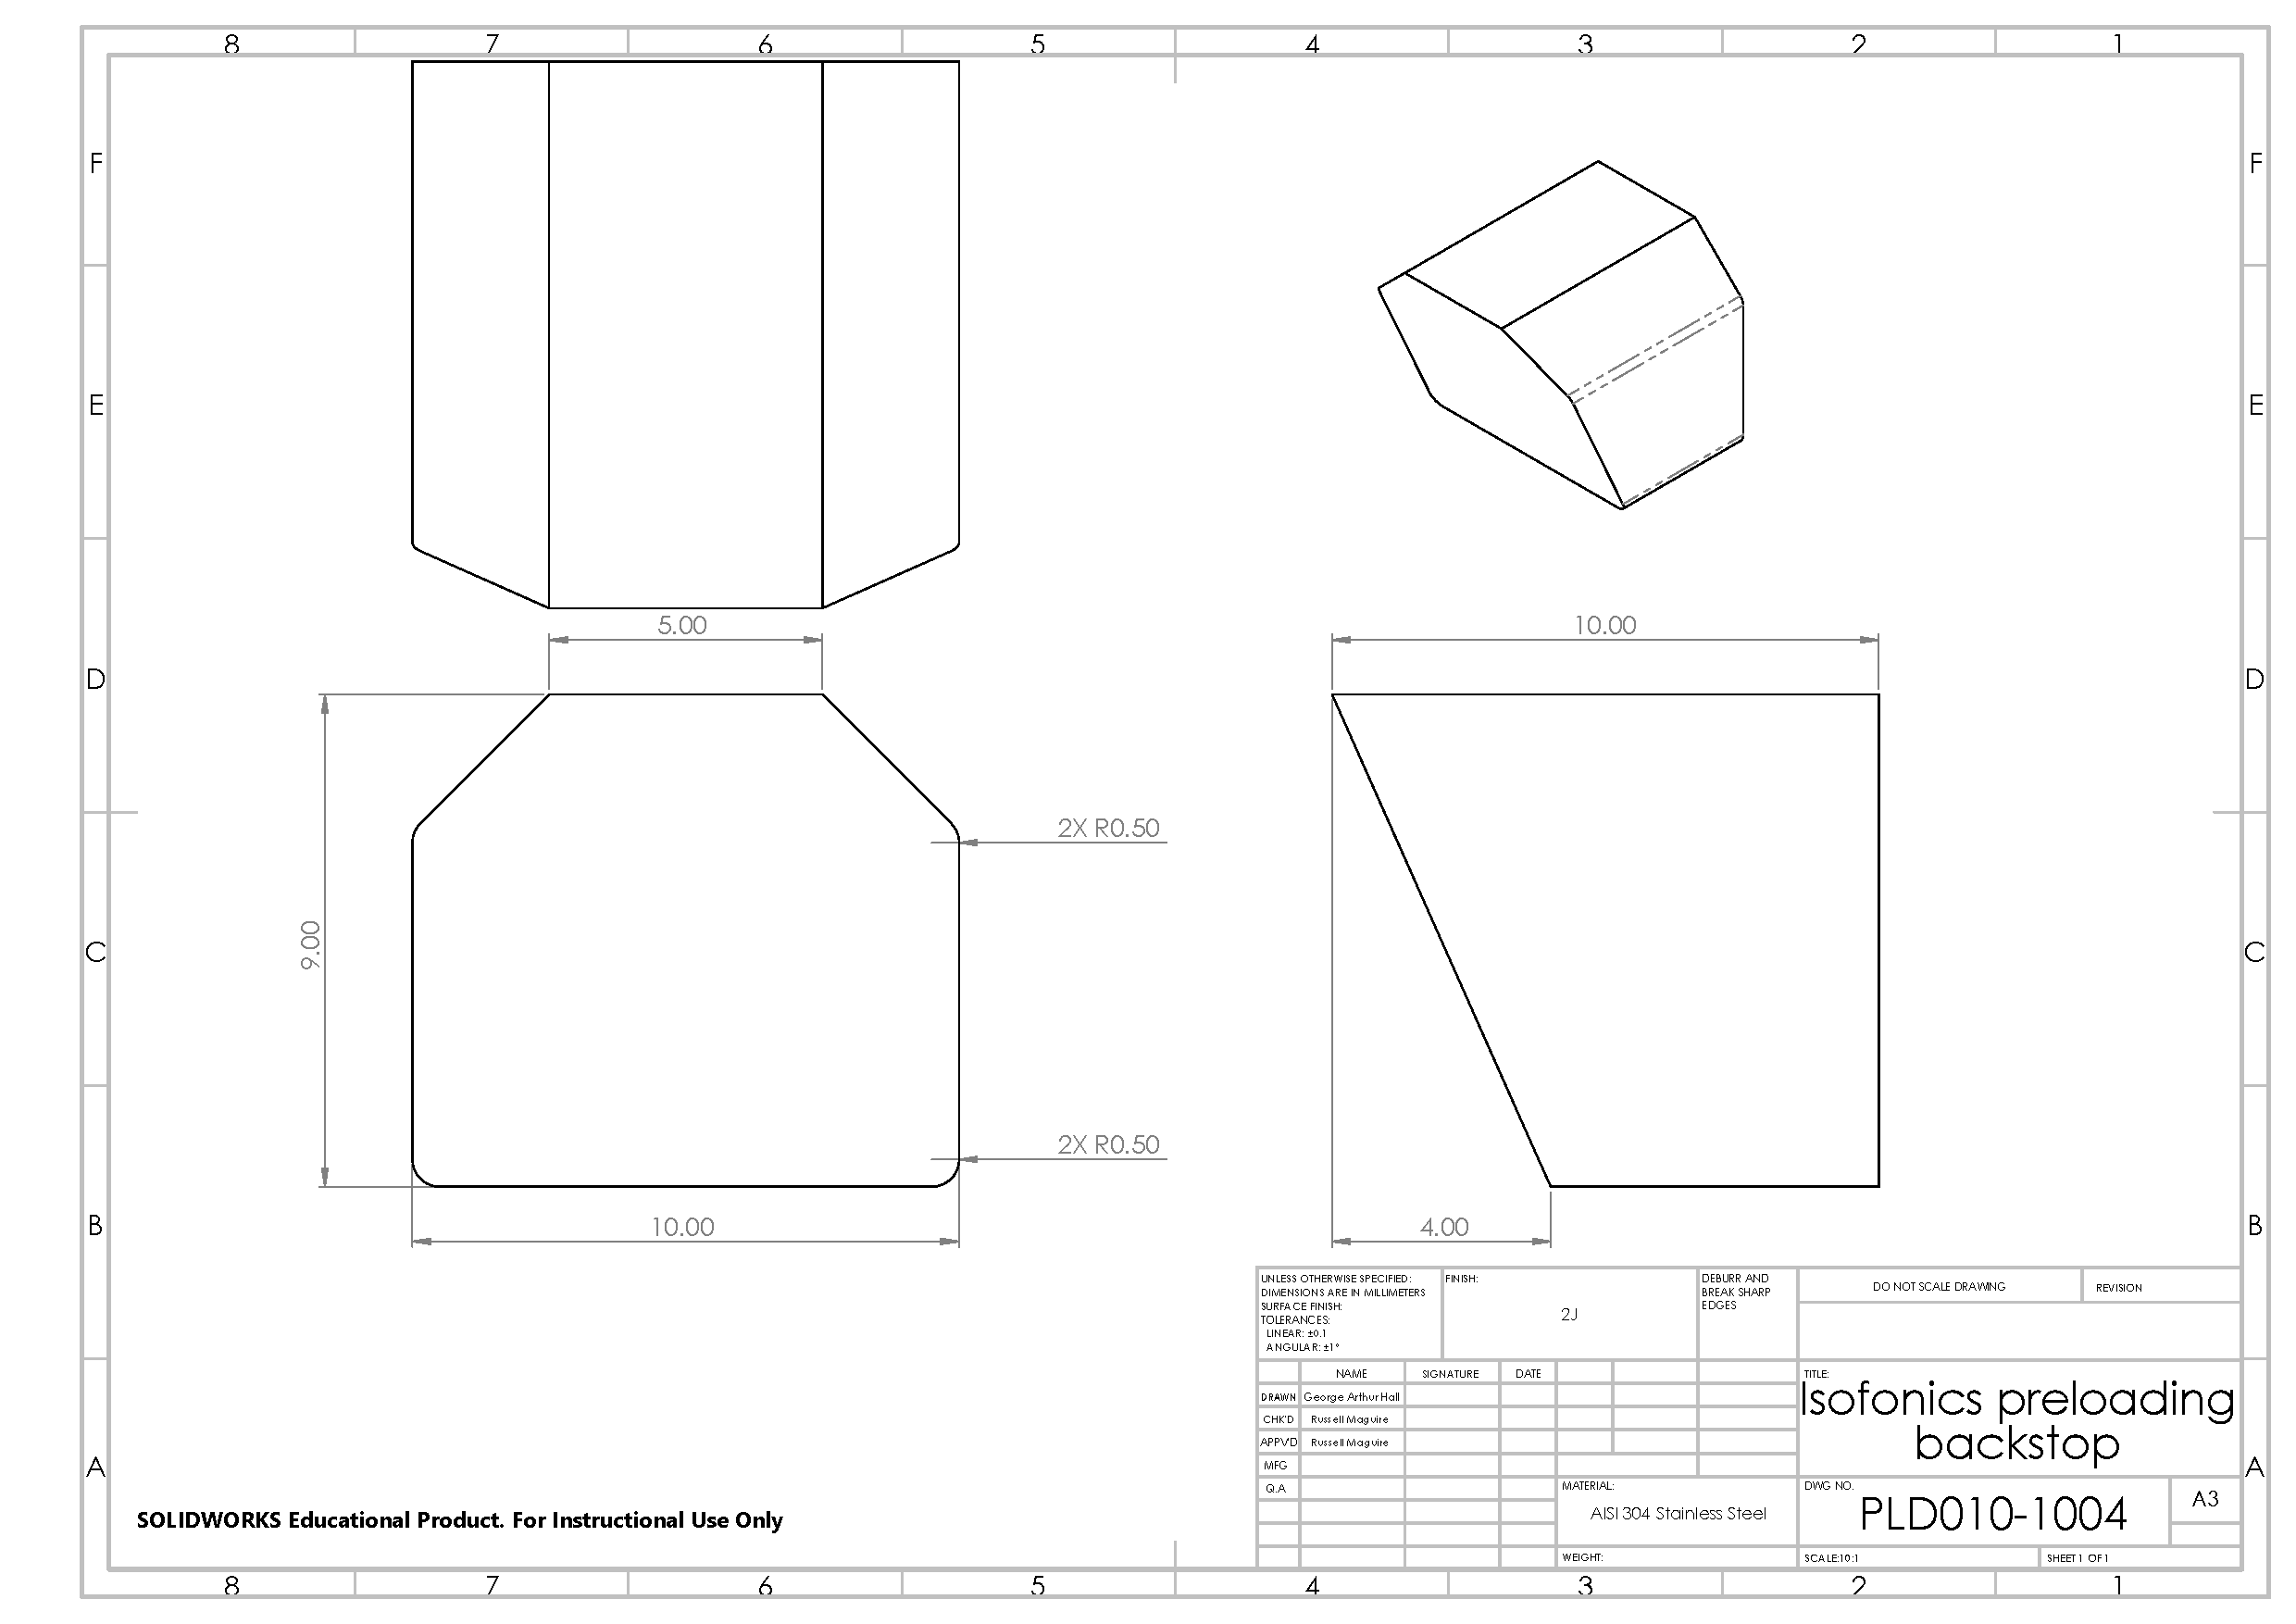
\includepdf[pages=-,fitpaper=true]{Images/Drawings/PLD010-1004.PDF}
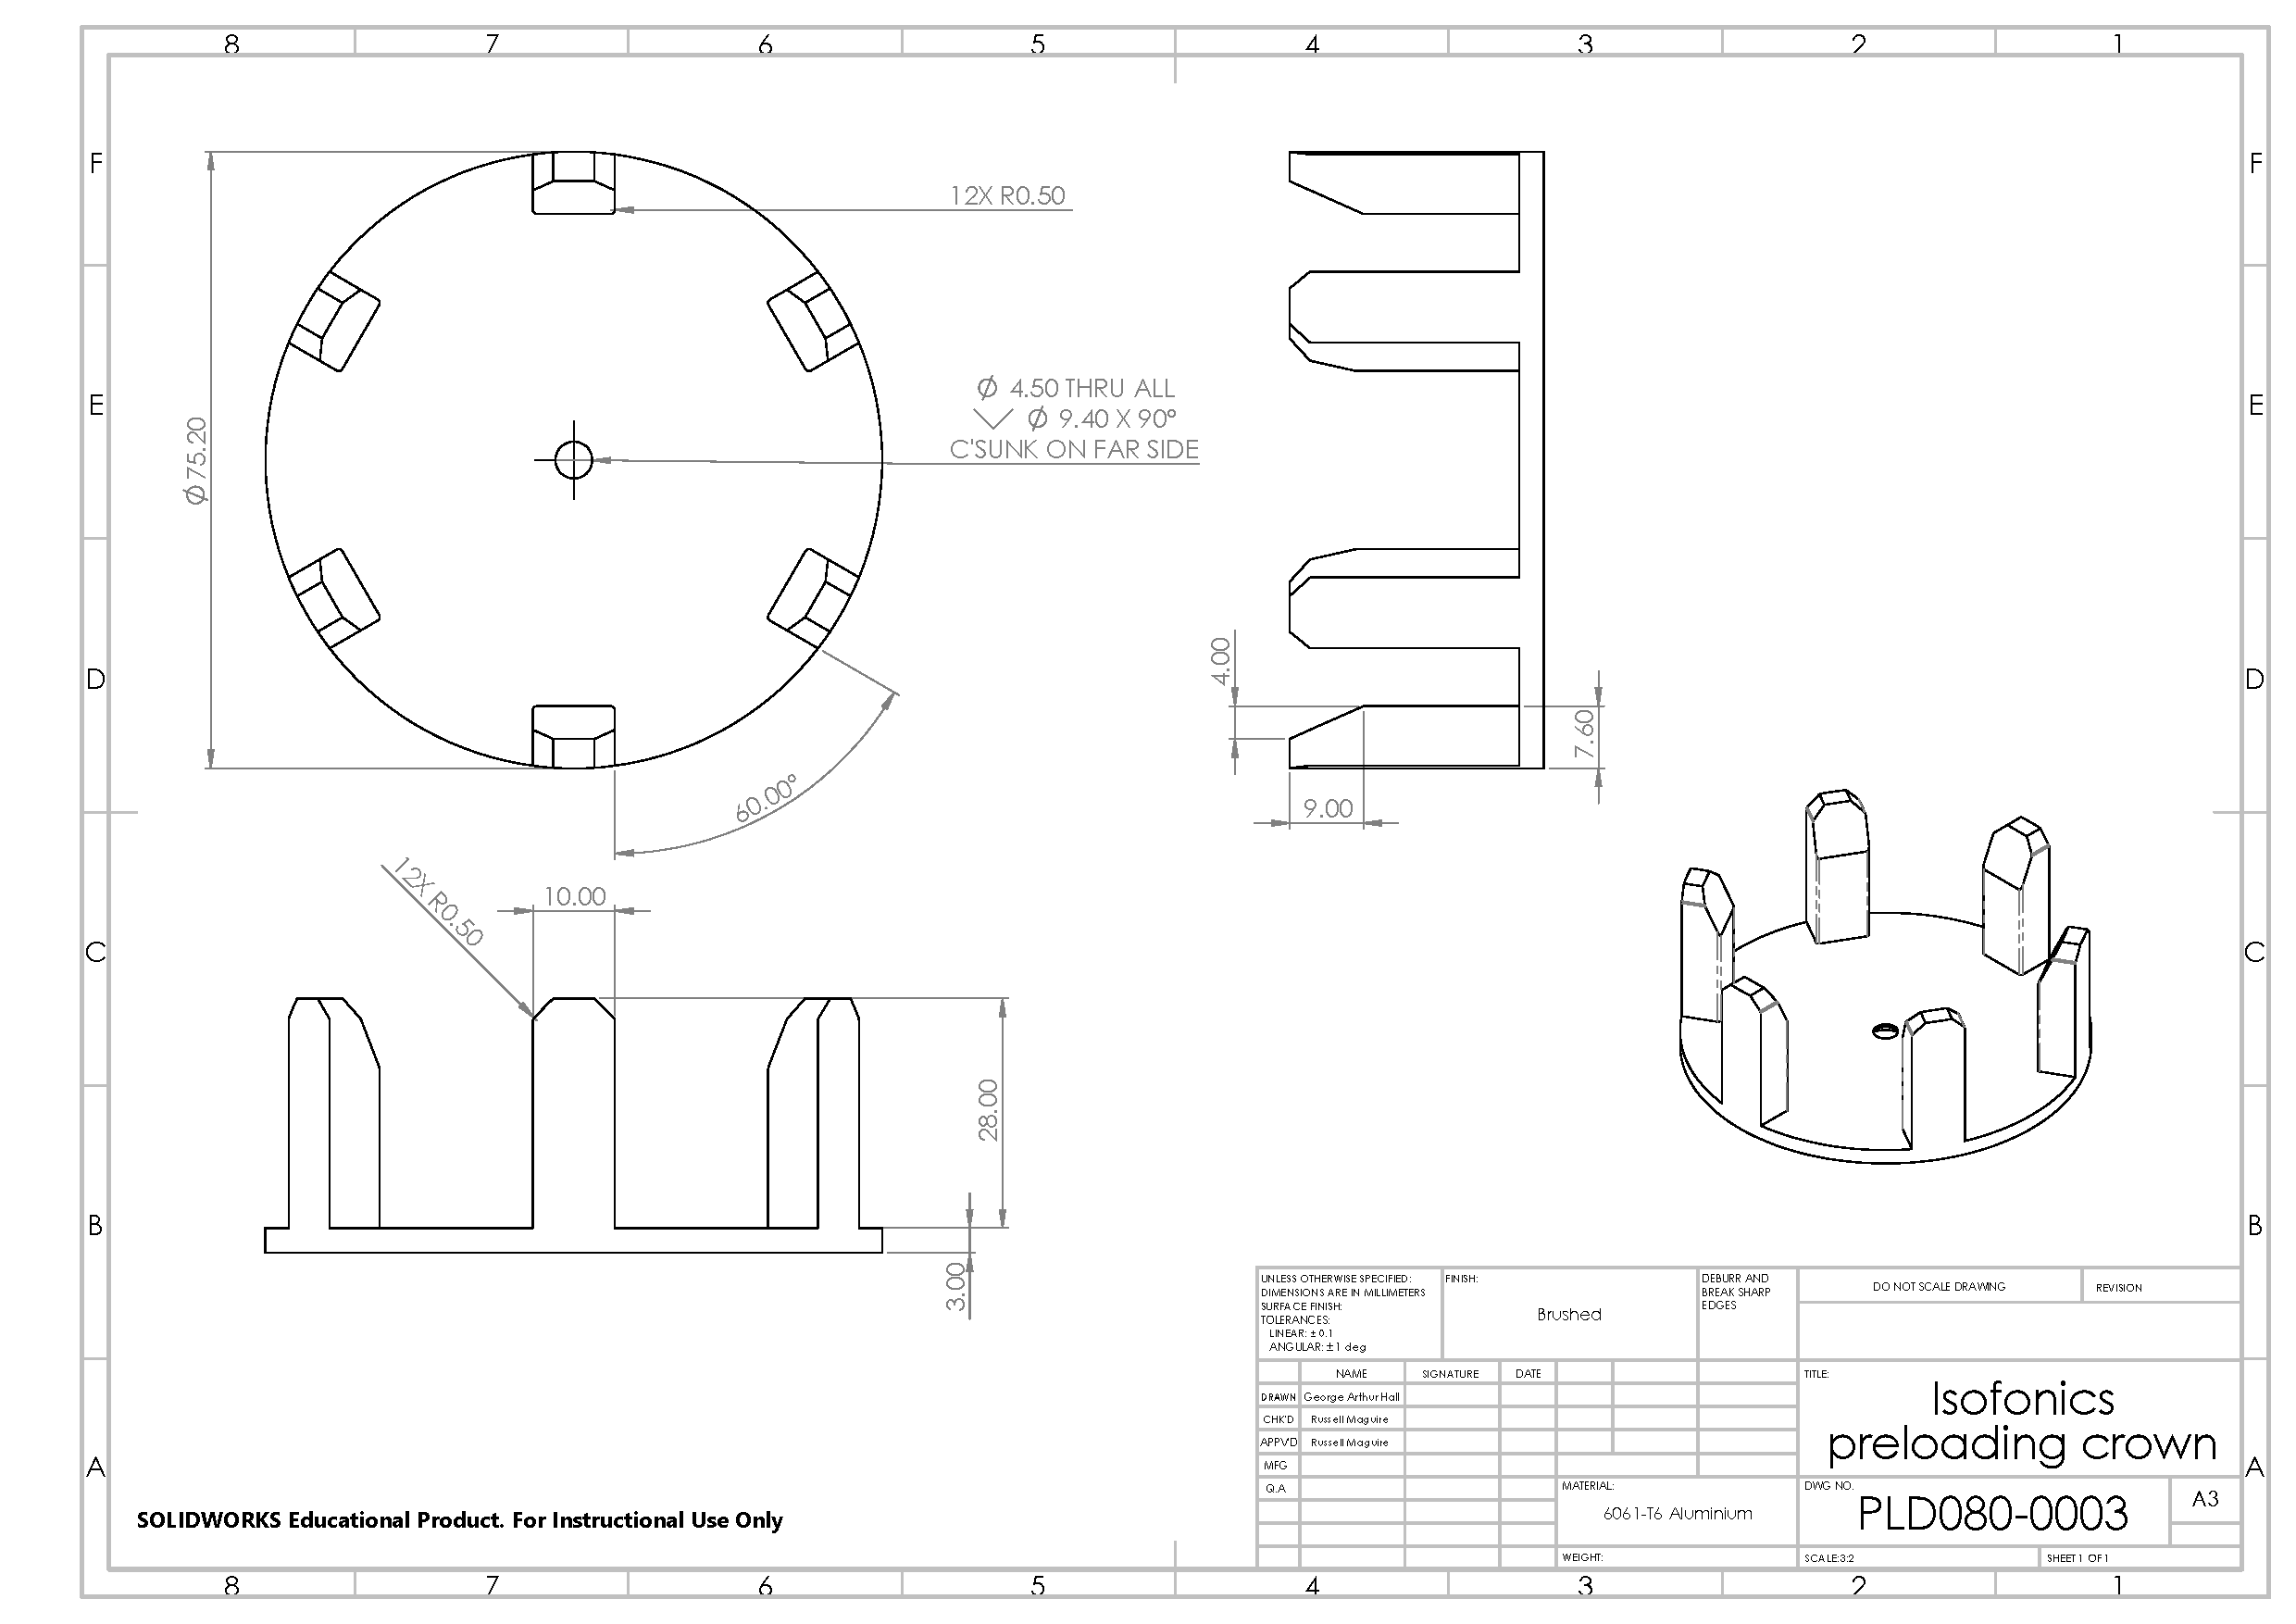
\includepdf[pages=-,fitpaper=true]{Images/Drawings/PLD080-0003.PDF}
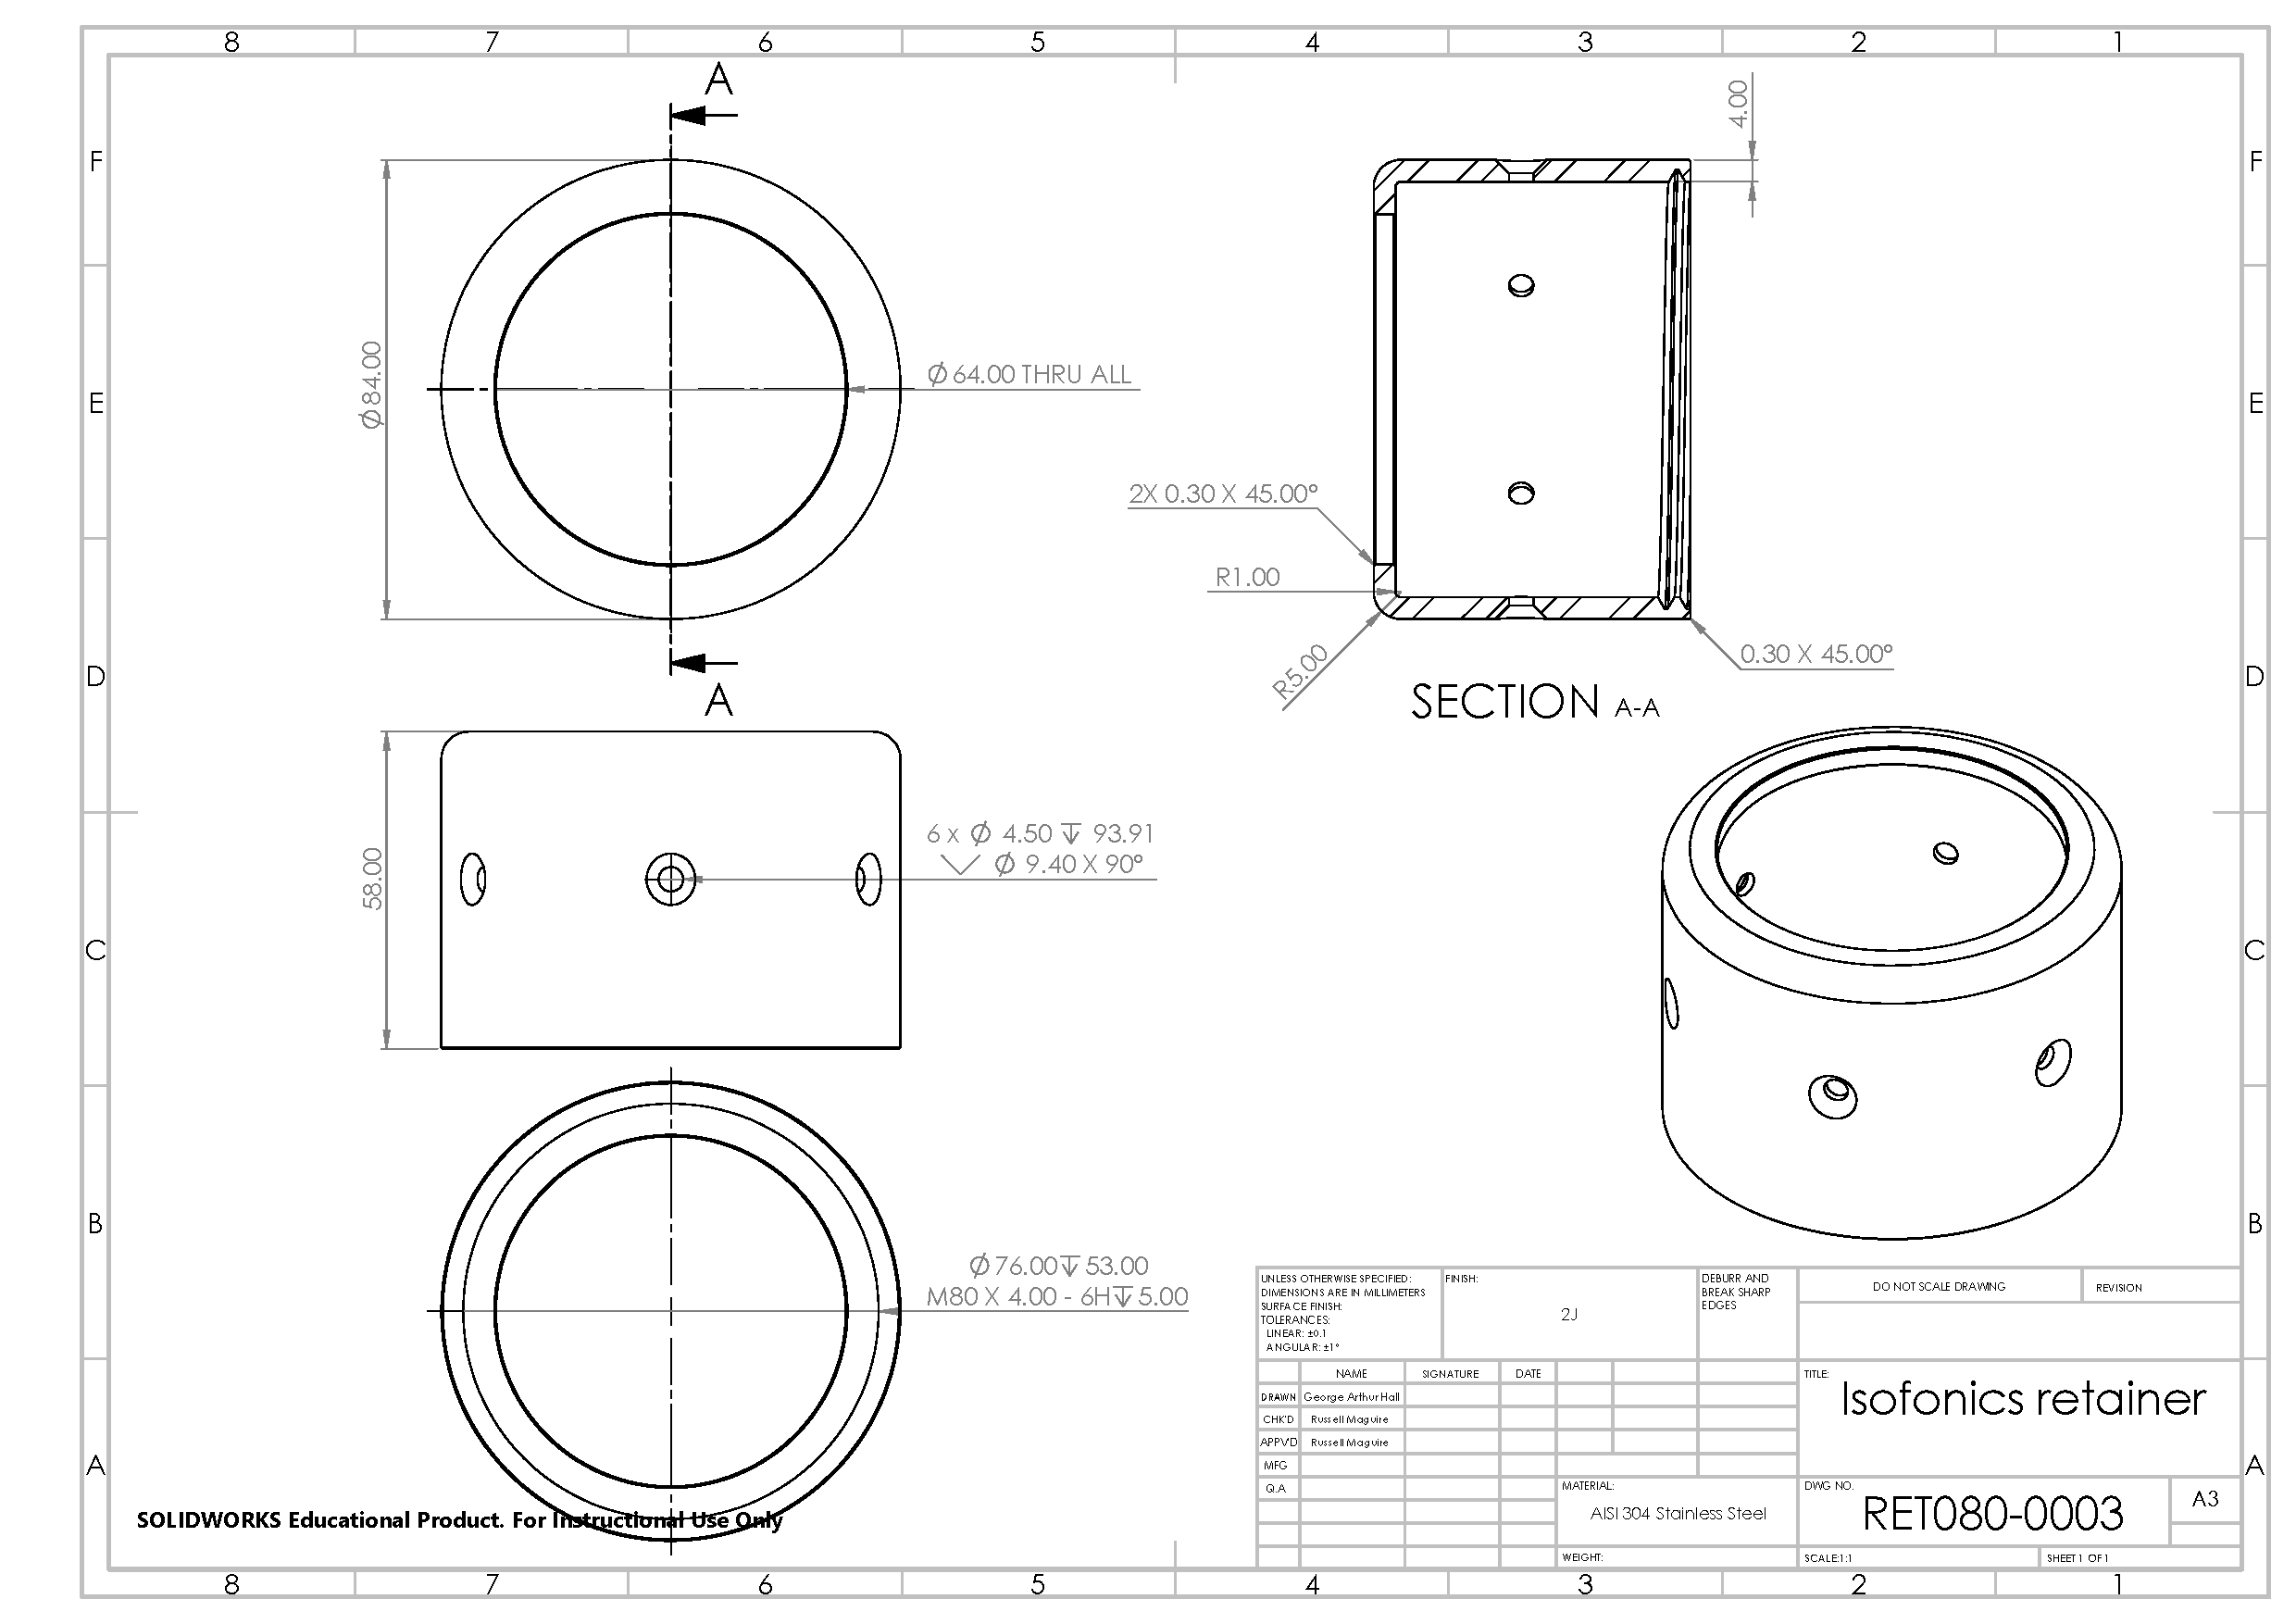
\includepdf[pages=-,fitpaper=true]{Images/Drawings/RET080-0003.PDF}
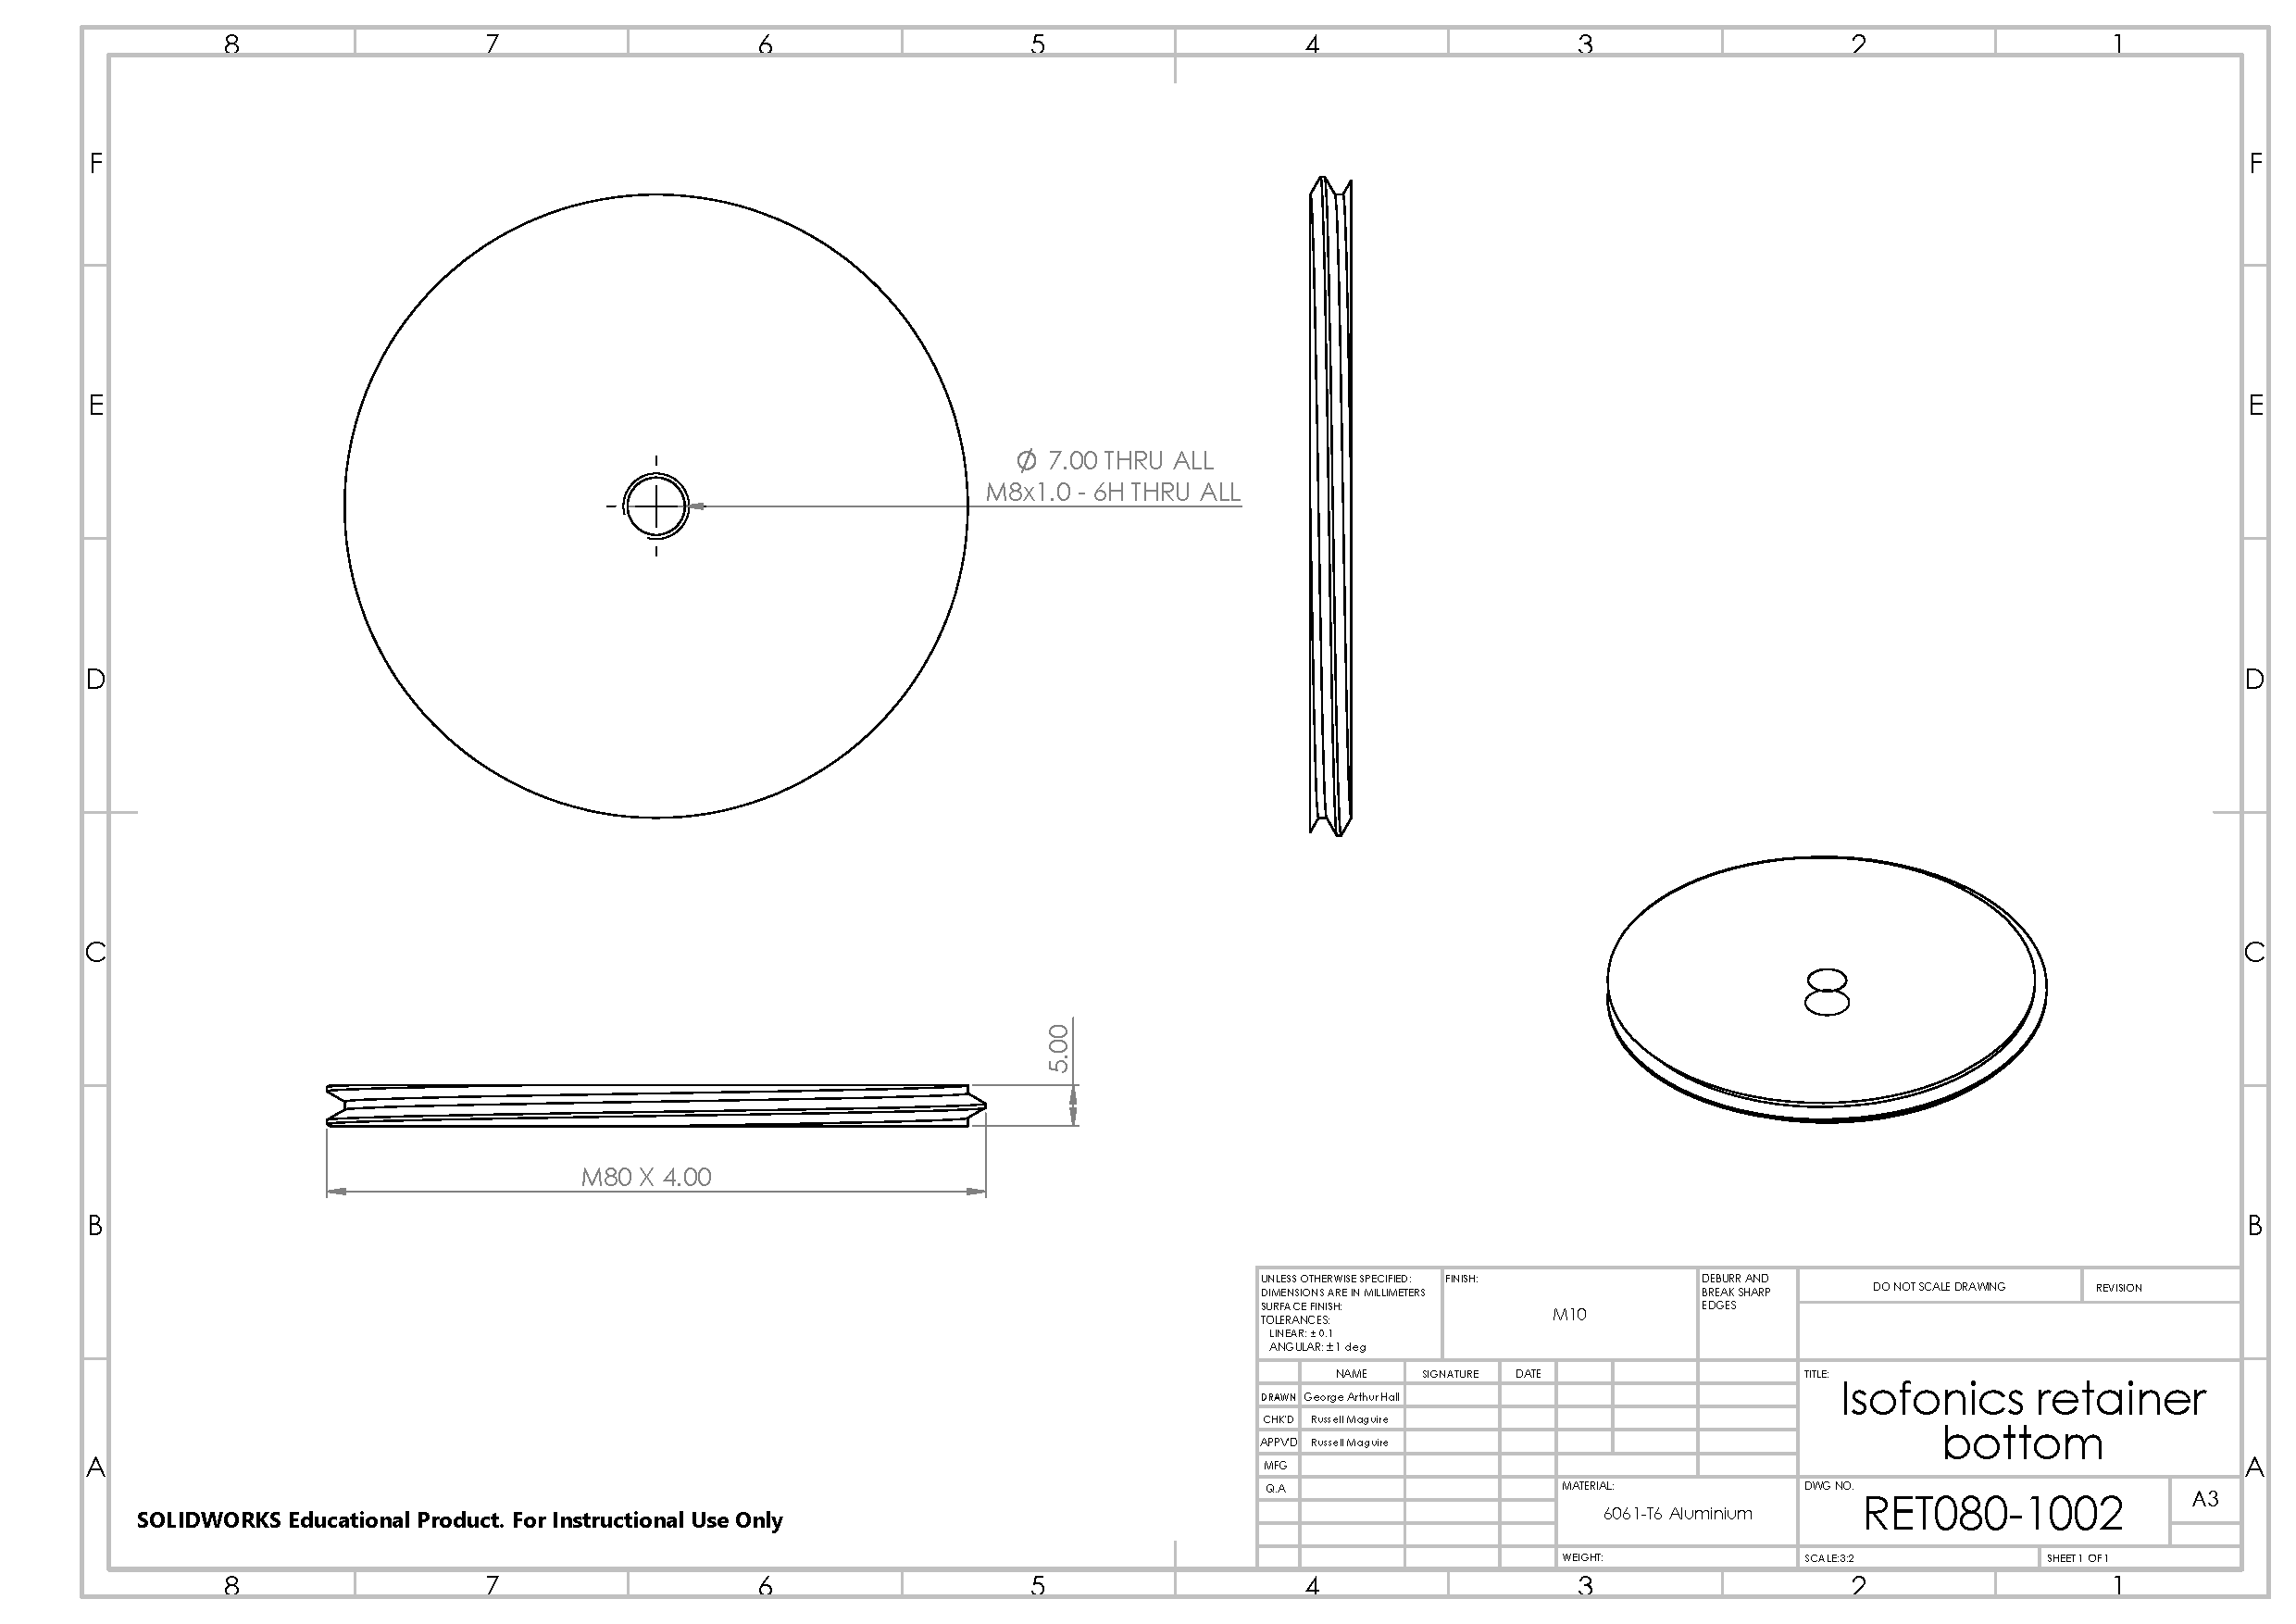
\includepdf[pages=-,fitpaper=true]{Images/Drawings/RET080-1002.PDF}
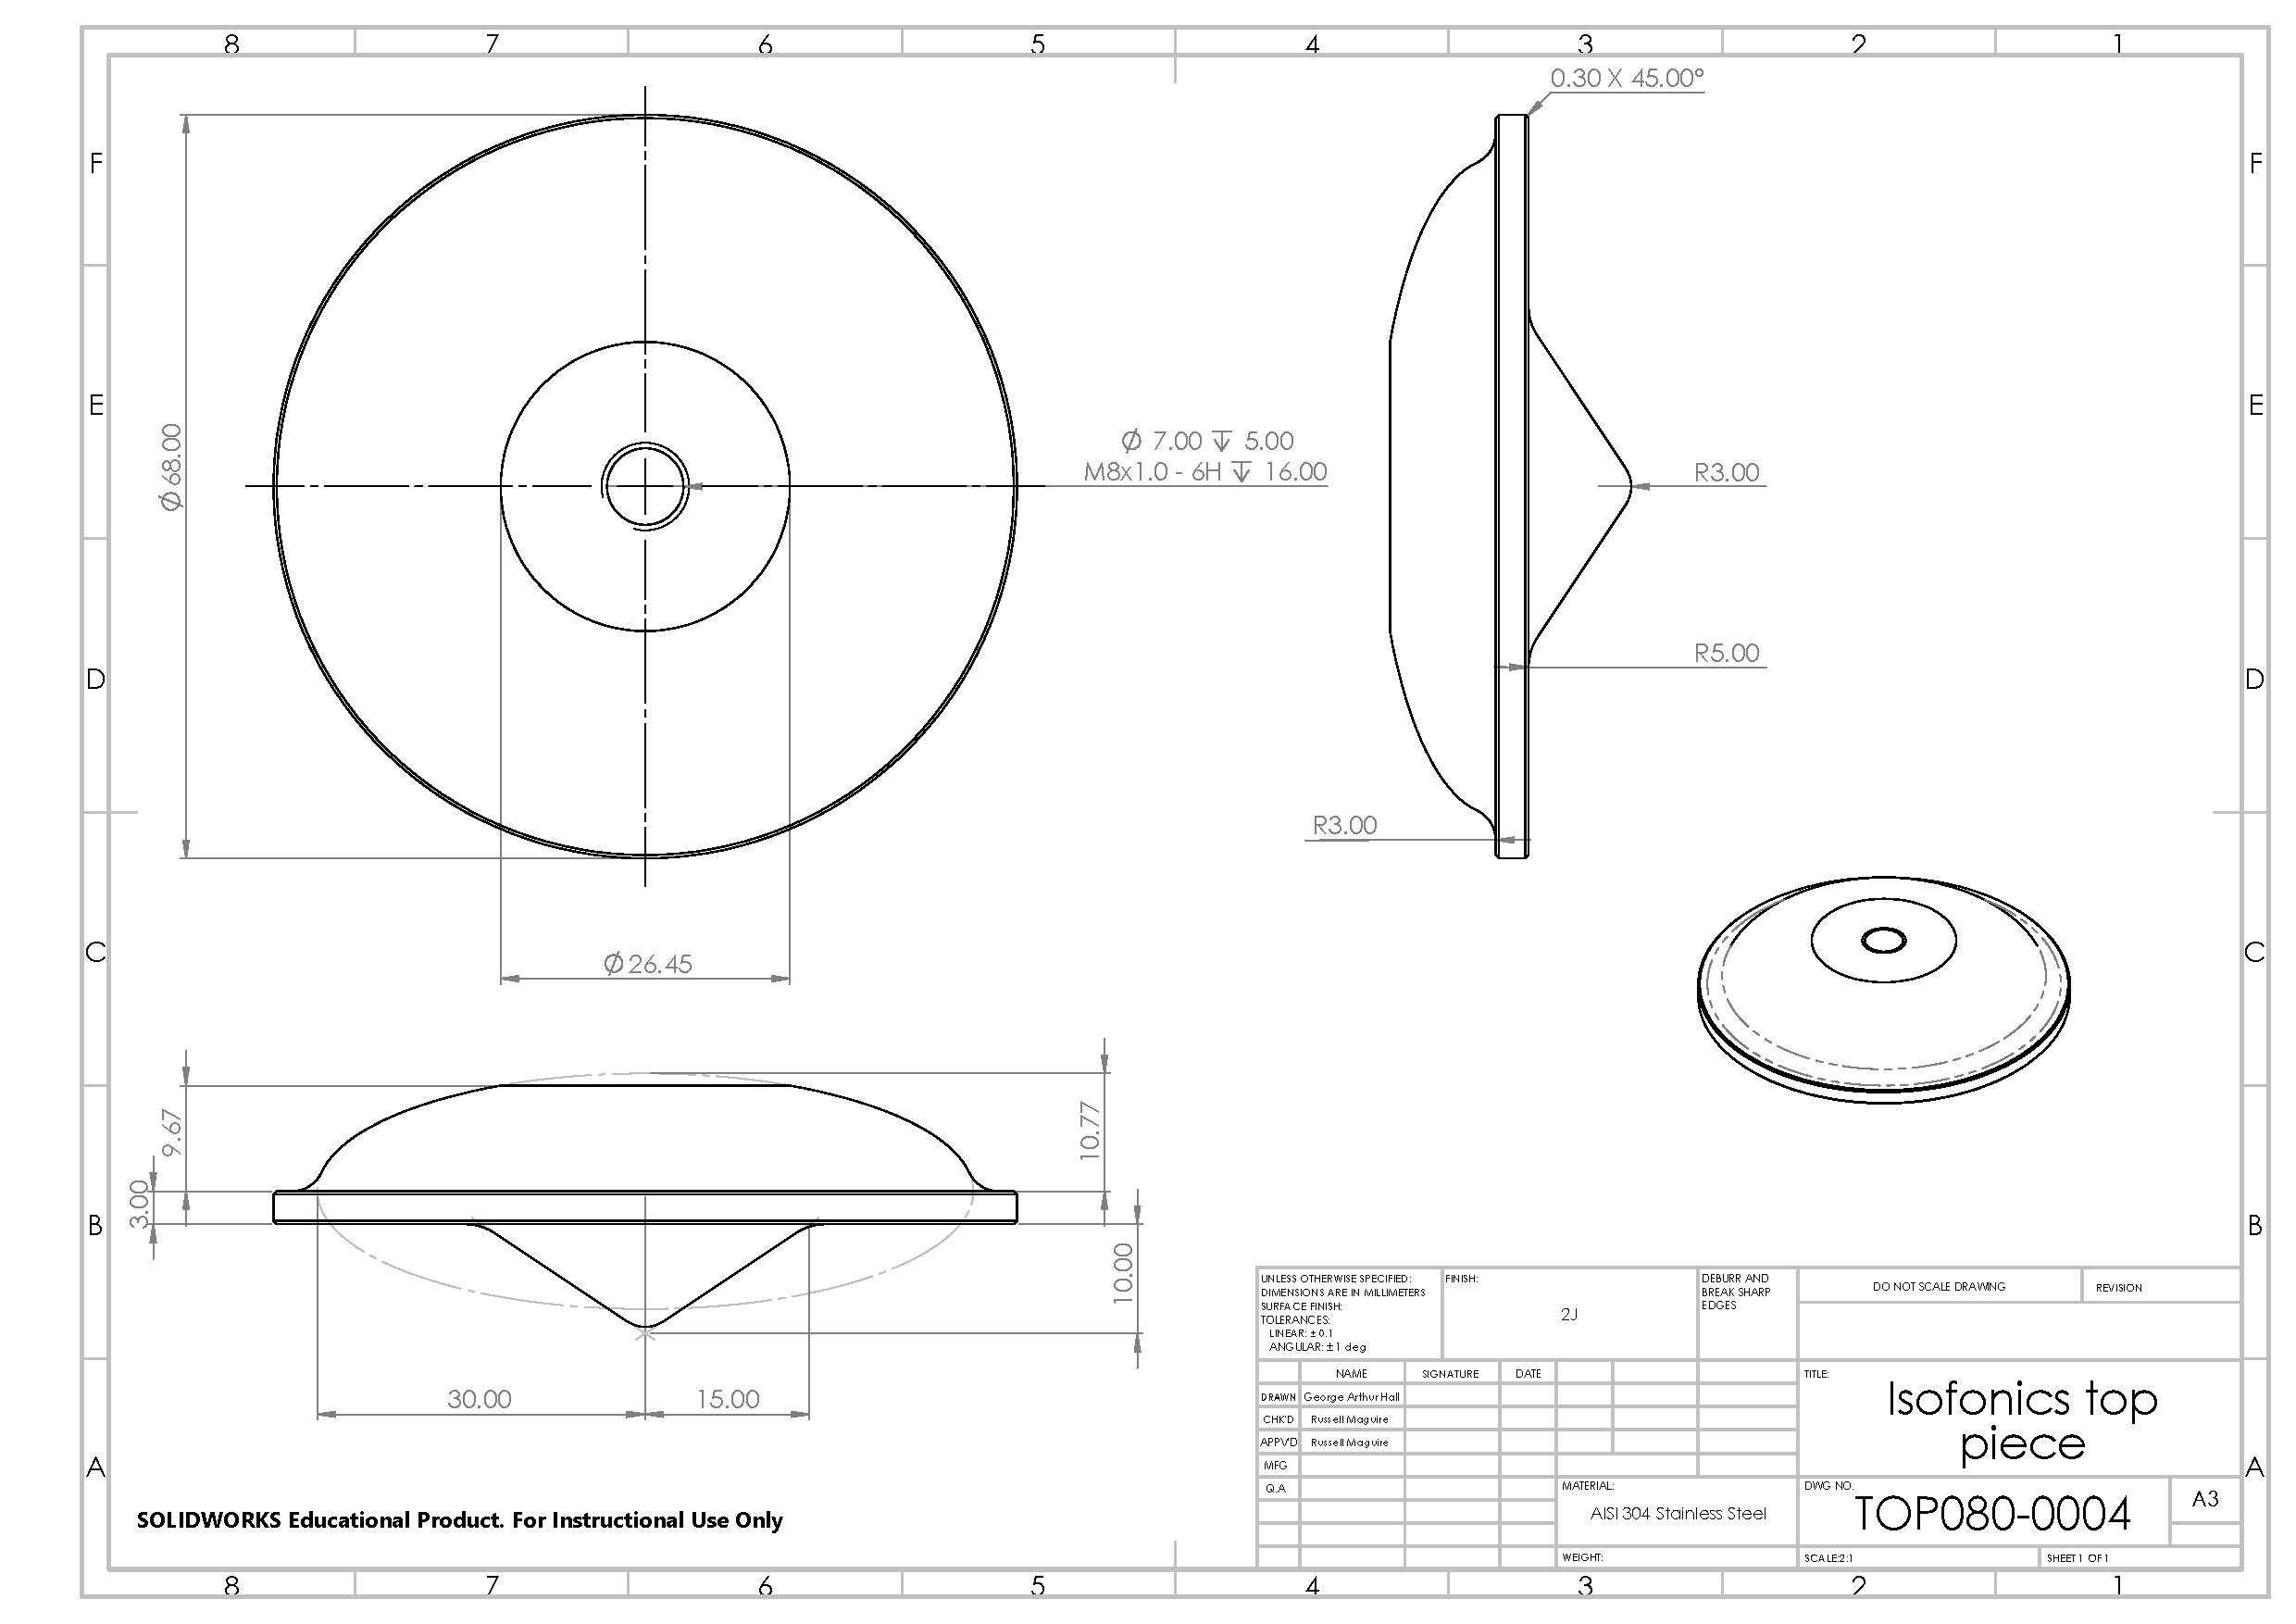
\includepdf[pages=-,fitpaper=true]{Images/Drawings/TOP080-0004.PDF}
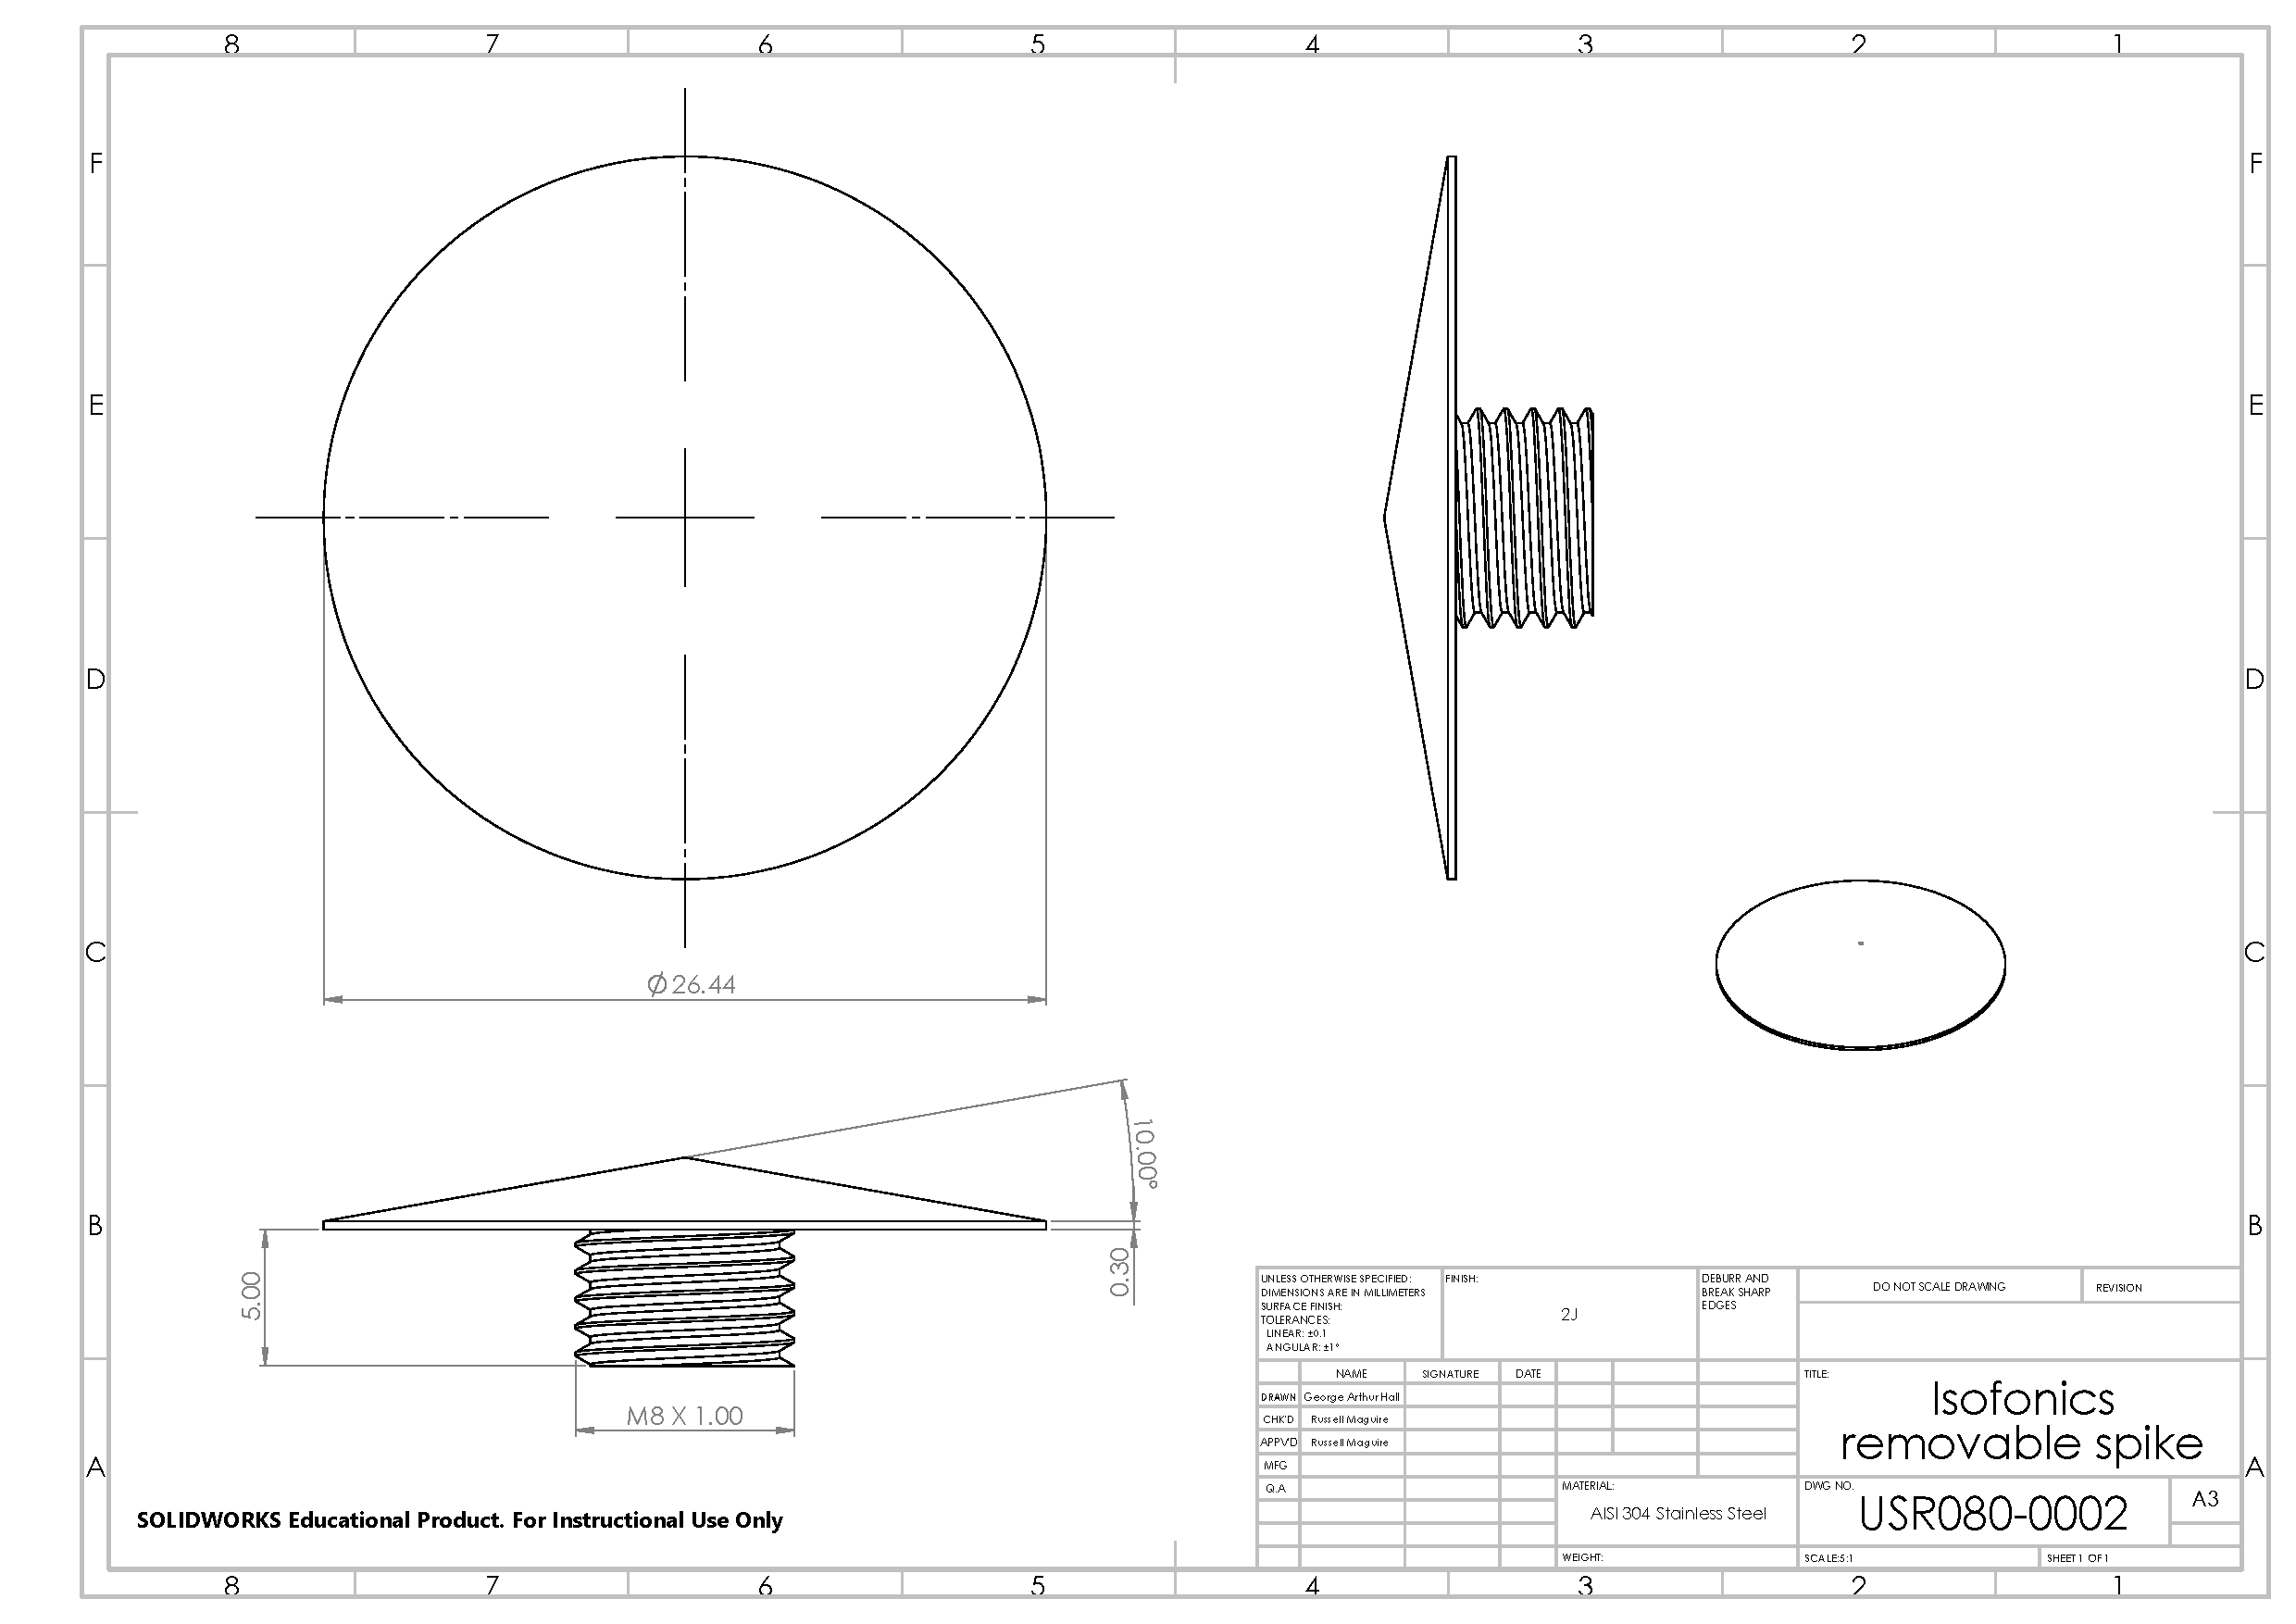
\includepdf[pages=-,fitpaper=true]{Images/Drawings/USR080-0002.PDF}
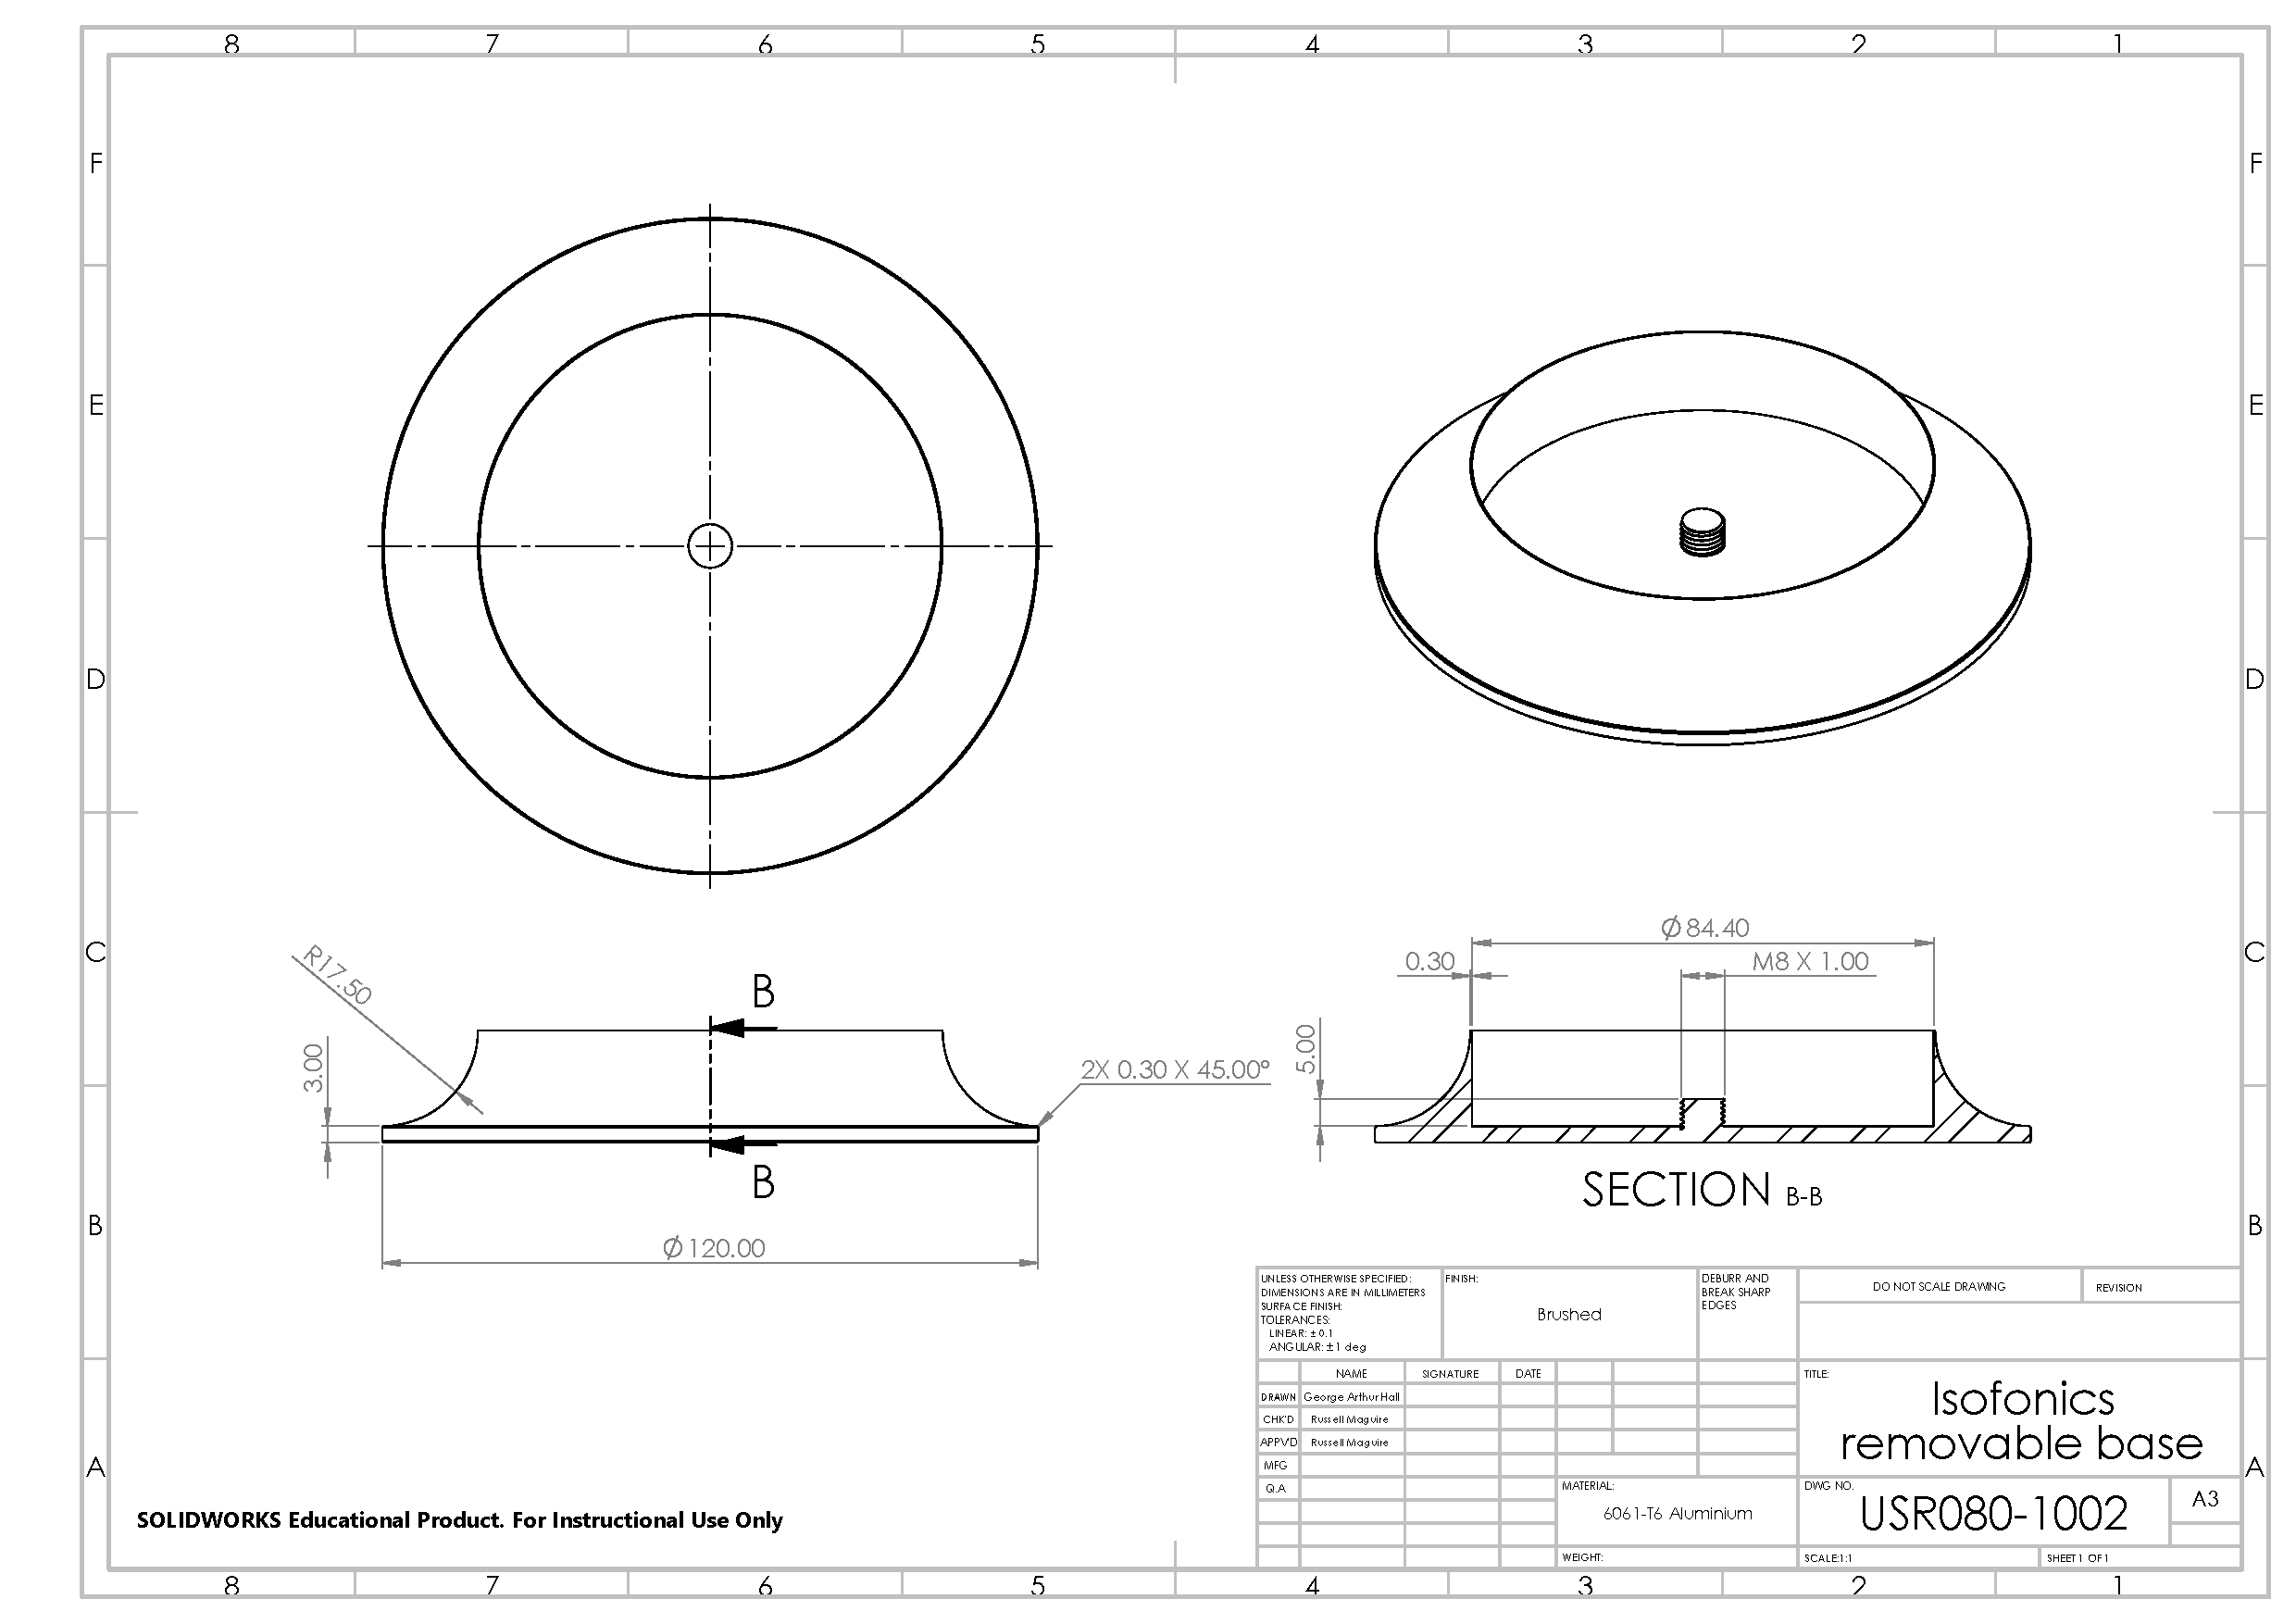
\includepdf[pages=-,fitpaper=true]{Images/Drawings/USR080-1002.PDF}

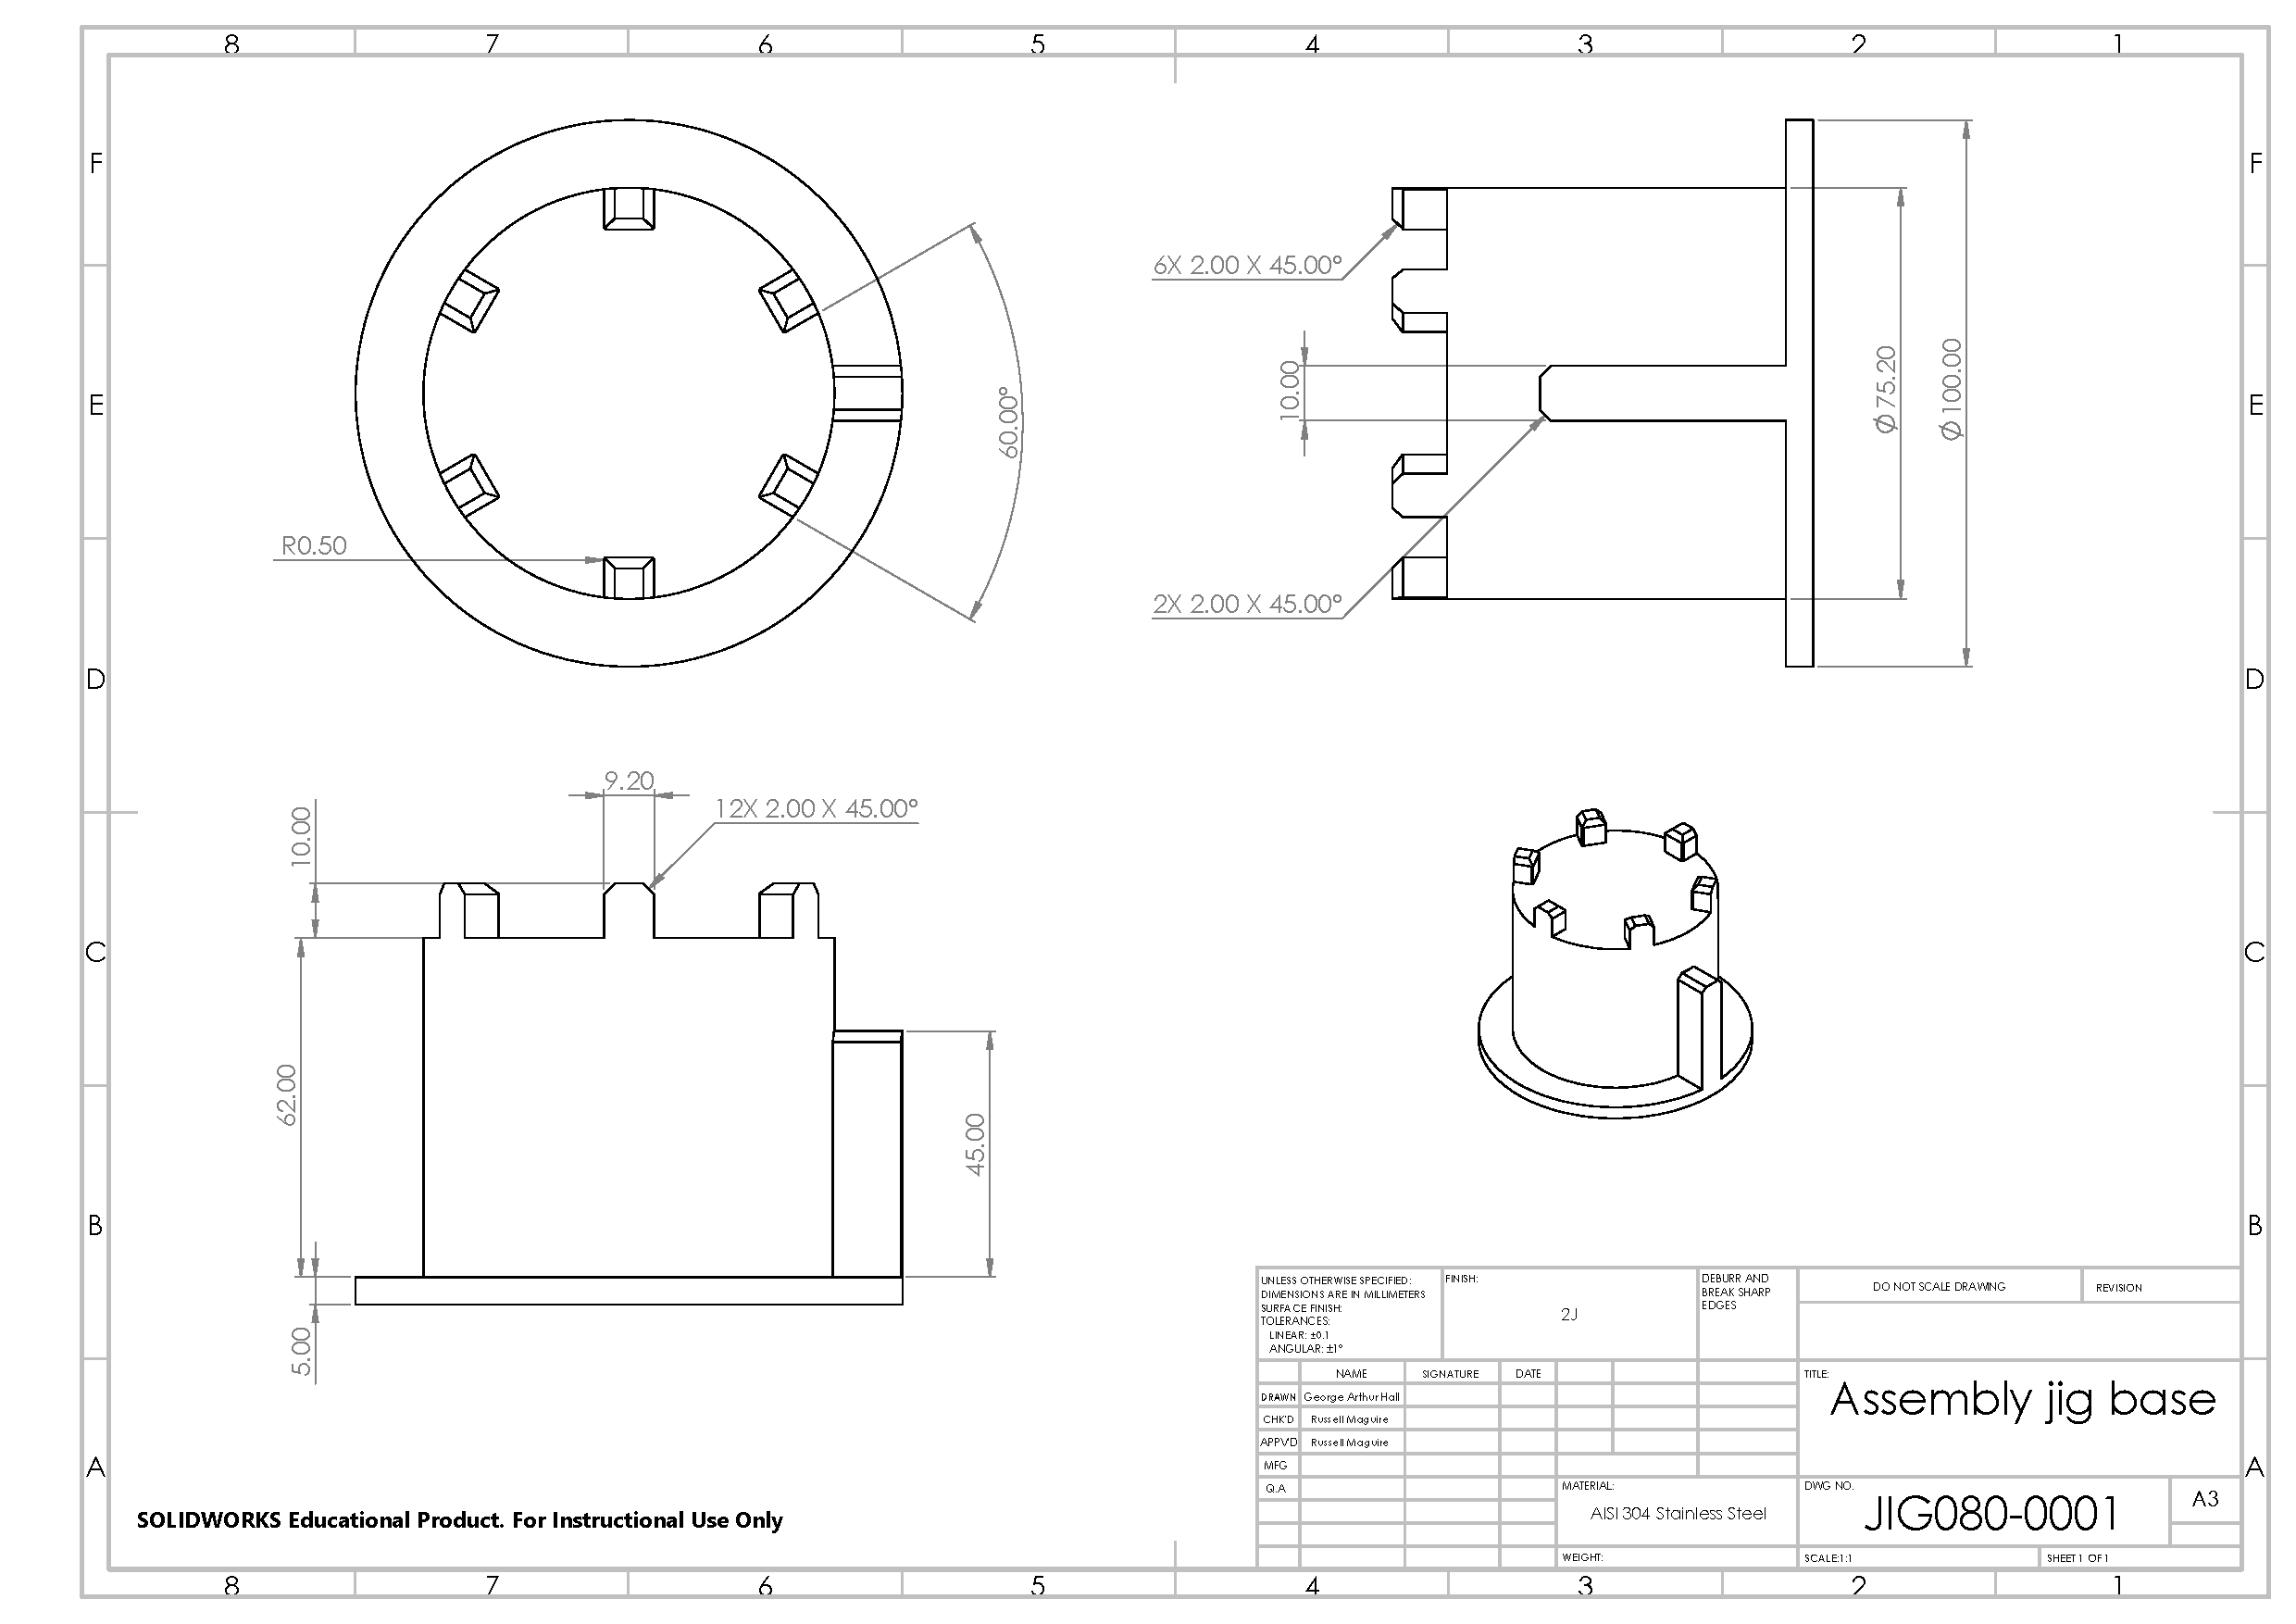
\includepdf[pages=-,fitpaper=true]{Images/jig/JIG080-0001.PDF}
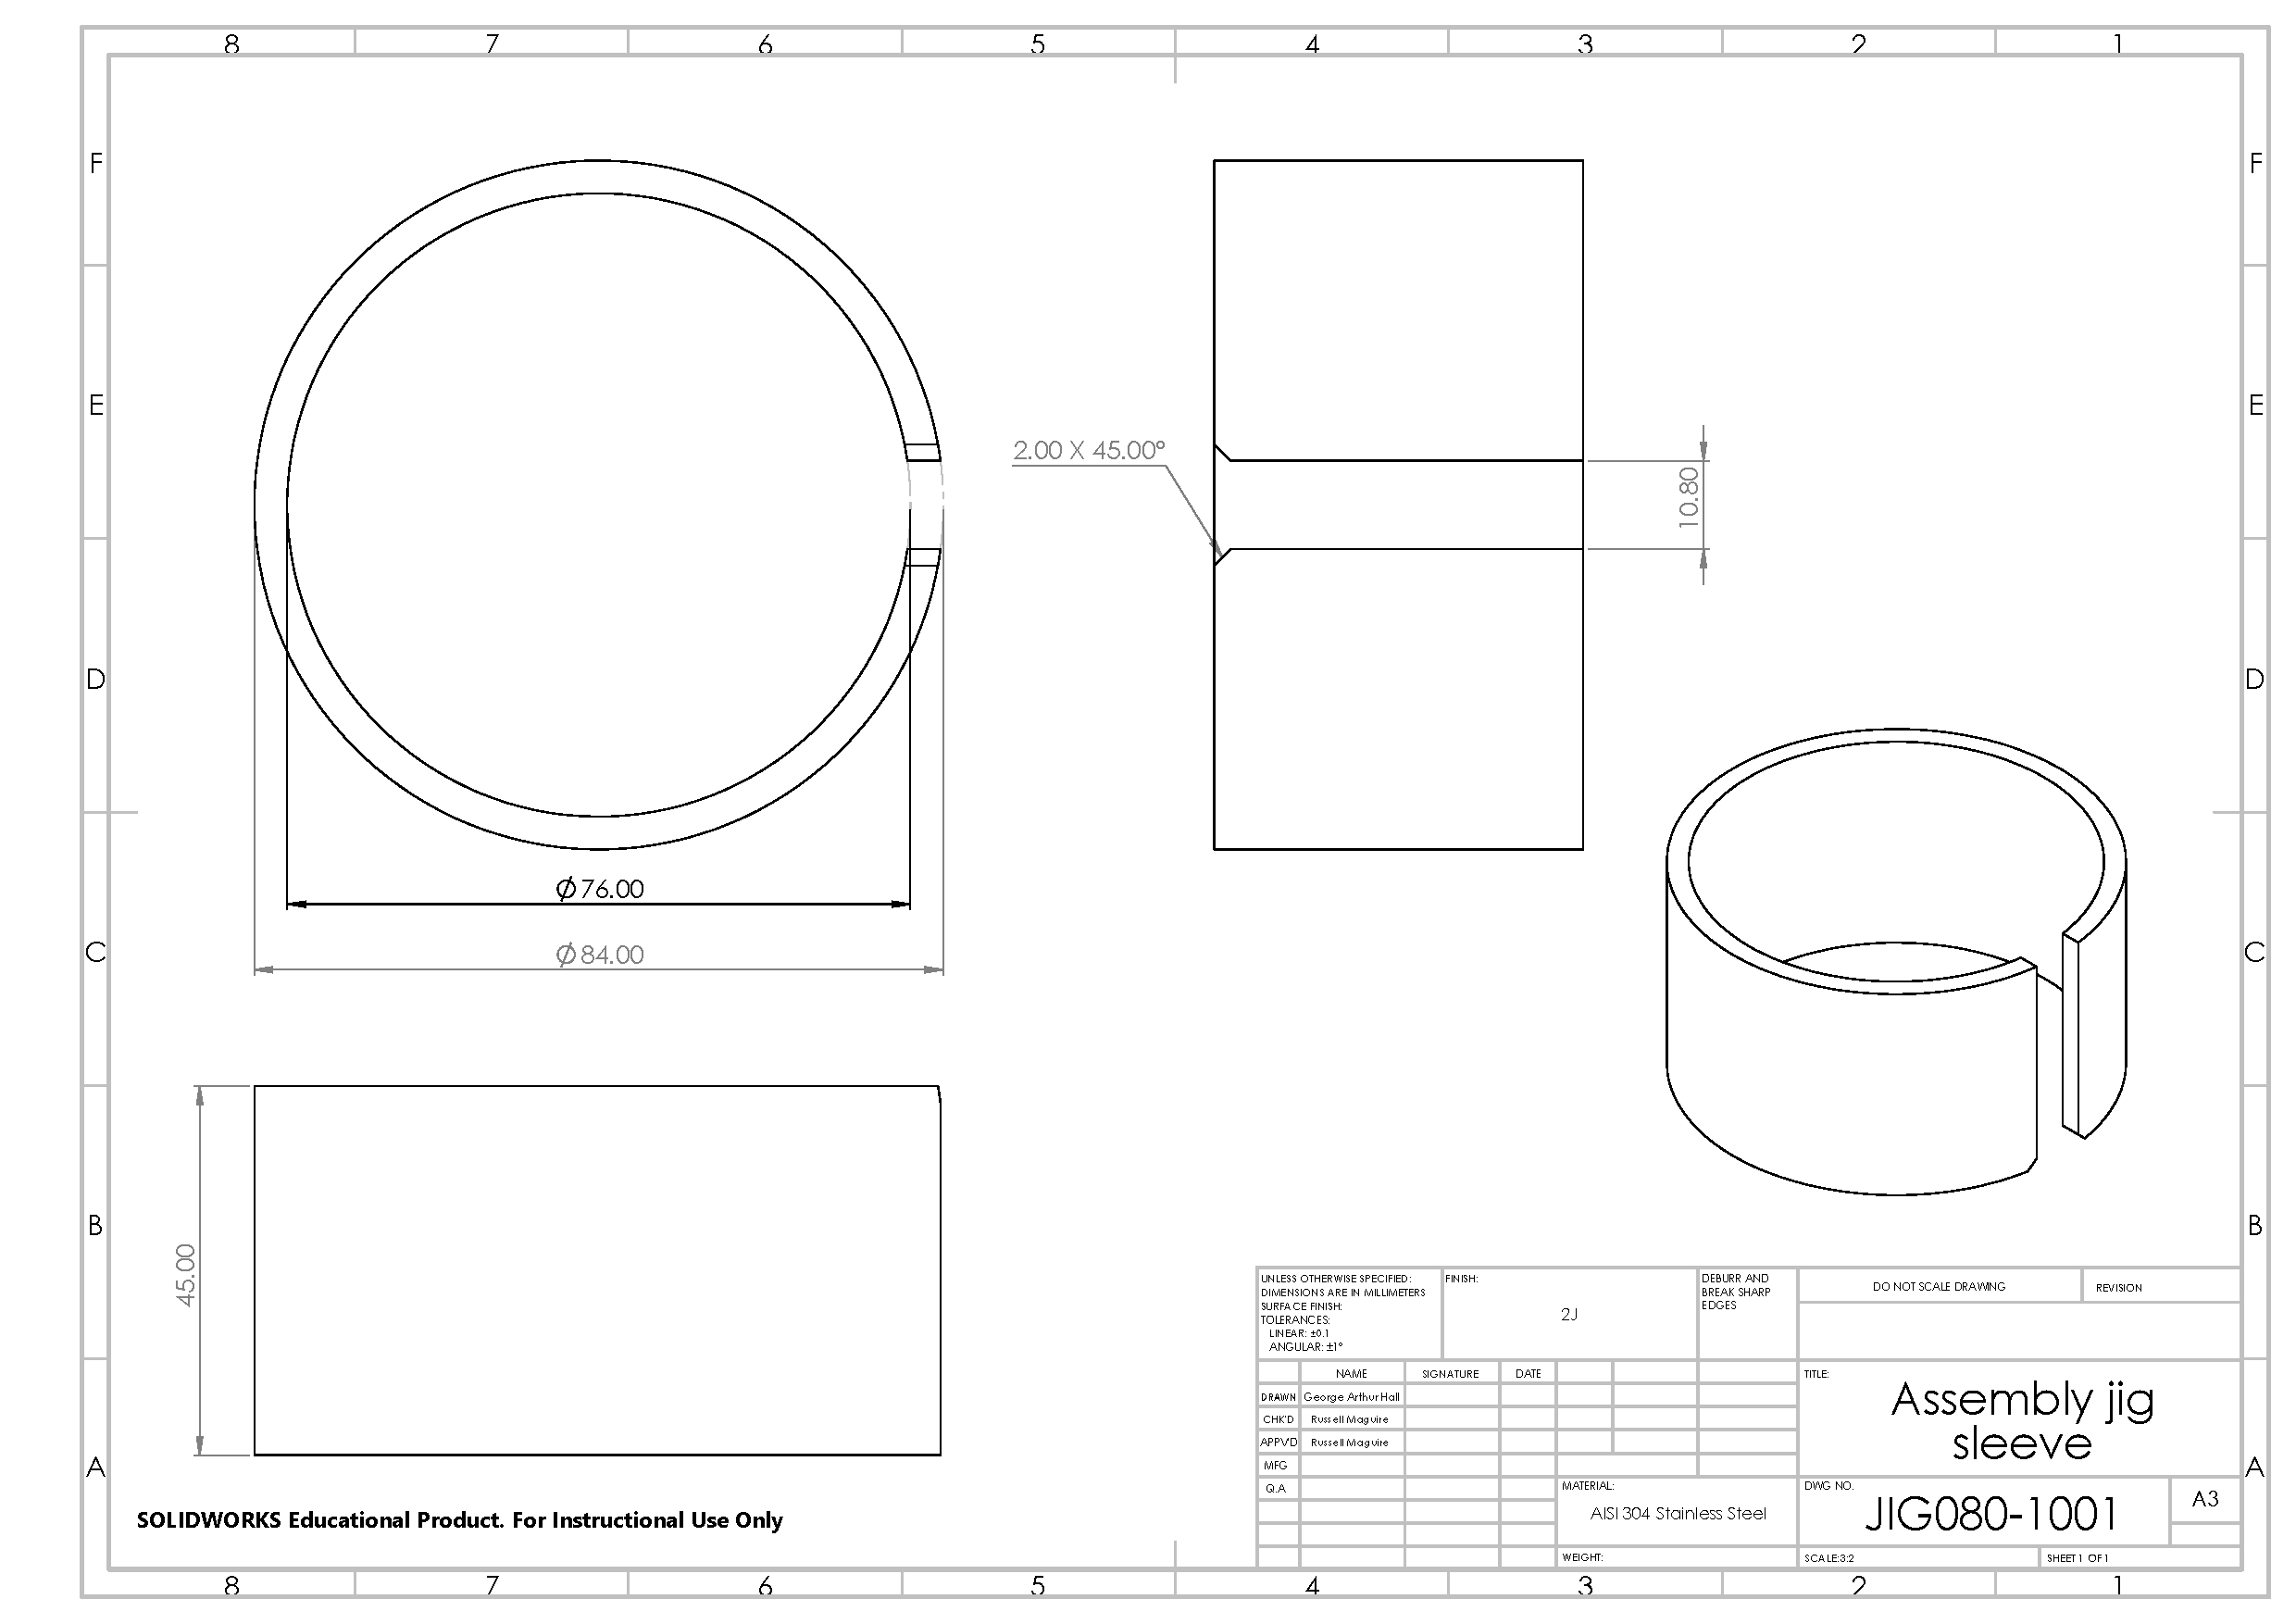
\includepdf[pages=-,fitpaper=true]{Images/jig/JIG080-1001.PDF}

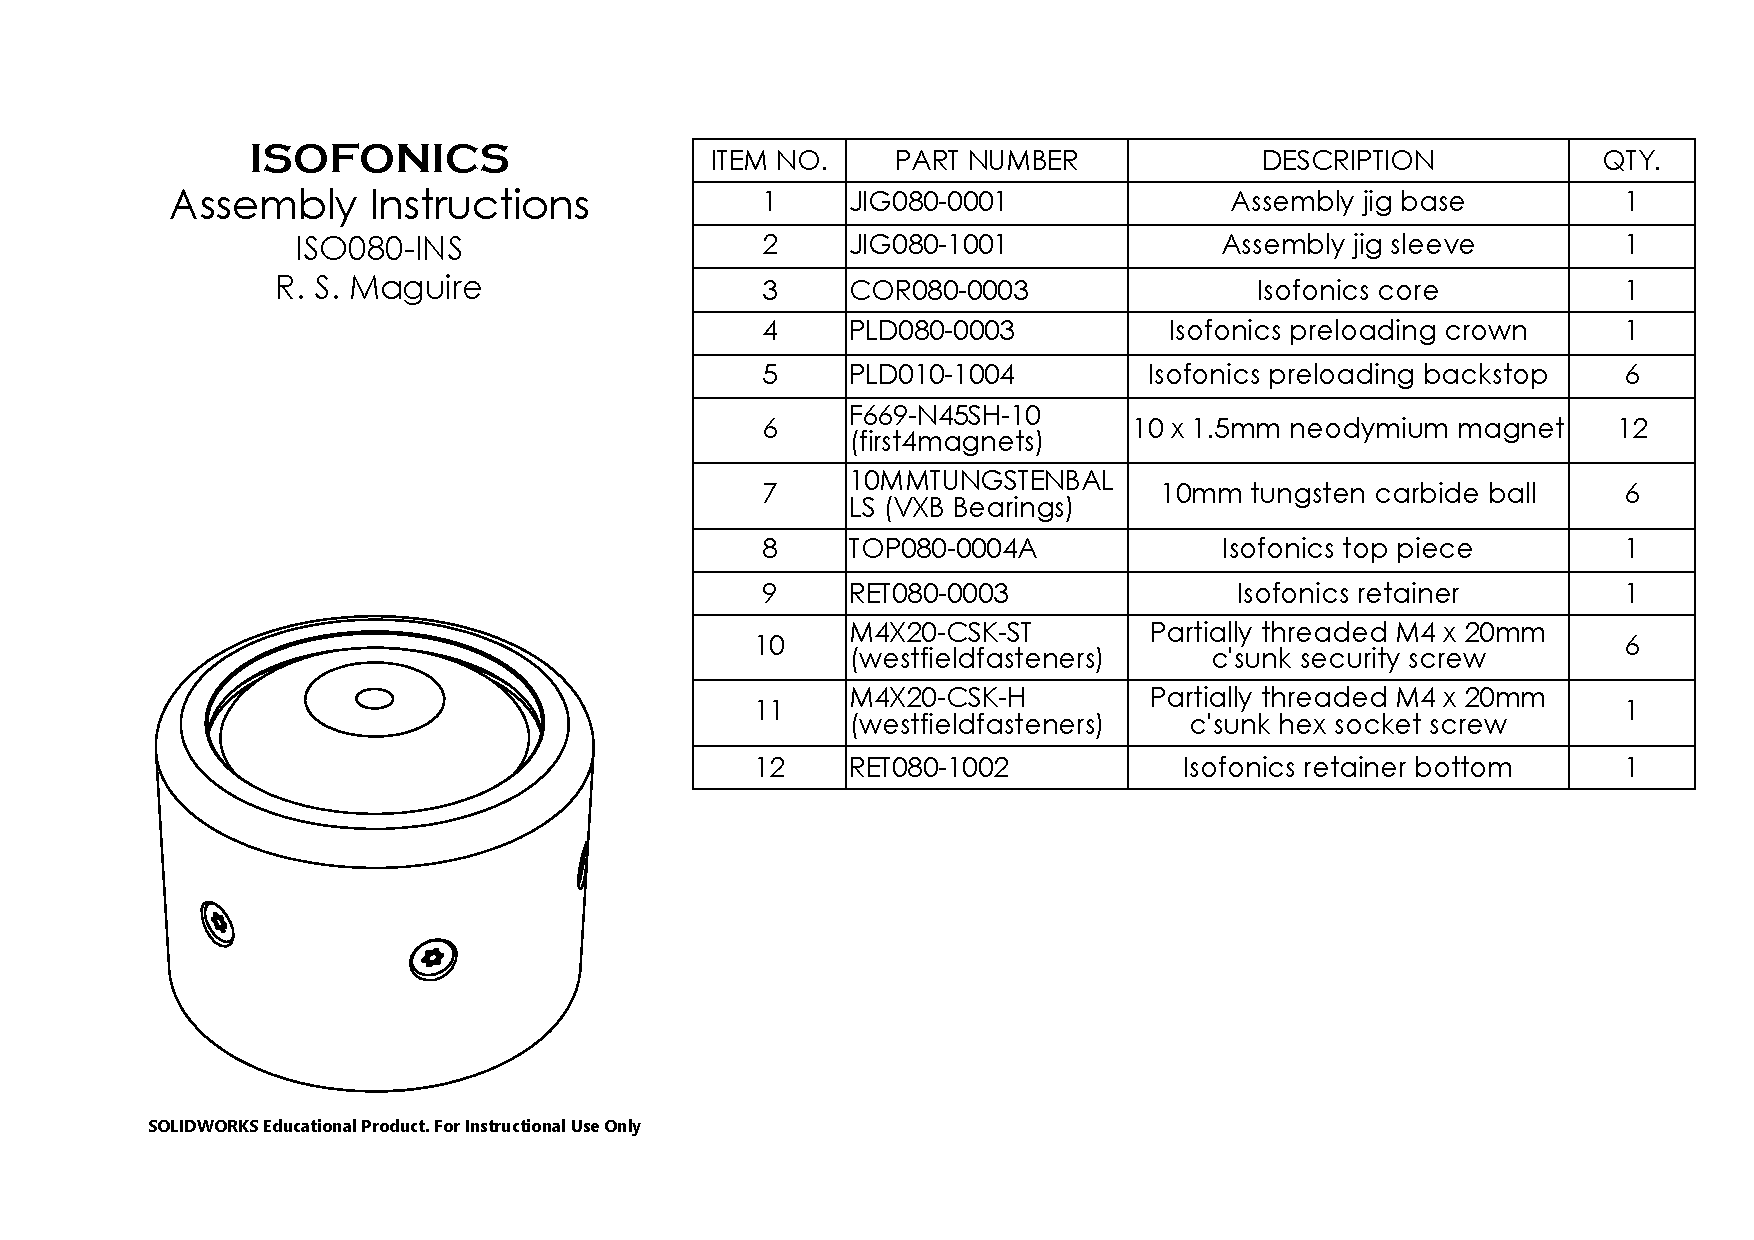
\includepdf[pages=-,fitpaper=true]{Images/jig/ISO080-INS.PDF}



\end{document}